% Тип документа
\documentclass[a4paper,12pt]{extarticle}

% Шрифты, кодировки, символьные таблицы, переносы
% \usepackage{cmap}
% \usepackage[T2A]{fontenc}
\usepackage[utf8]{inputenc}
\usepackage[russian]{babel}
% Это пакет -- хитрый пакет, он нужен но не нужен
\usepackage[mode=buildnew]{standalone}

\usepackage
	{
		% Дополнения Американского математического общества (AMS)
		amssymb,
		amsfonts,
		amsmath,
		amsthm,
		% Пакет для физических текстов
		physics,
		% misccorr,
		% 
		% Графики и рисунки
		wrapfig,
		graphicx,
		subcaption,
		float,
		tikz,
		tikz-3dplot,
		caption,
		csvsimple,
		color,
		booktabs,
		geometry,
		% 
		% Таблицы, списки
		makecell,
		multirow,
		indentfirst,
		%
		% Интегралы и прочие обозначения
		ulem,
		esint,
		esdiff,
		% 
		% Колонтитулы
		fancyhdr,
	} 
    
\usepackage{mathtools}
% \mathtoolsset{showonlyrefs=true} 
\usepackage{pgfplots,pgfplotstable,booktabs,colortbl}
\usepackage{xcolor}
\usepackage{hyperref}
\usepackage{pythontex}
 % Цвета для гиперссылок
\definecolor{linkcolor}{HTML}{000000} % цвет ссылок
\definecolor{urlcolor}{HTML}{799B03} % цвет гиперссылок
 
\hypersetup{pdfstartview=FitH,linkcolor=linkcolor,urlcolor=urlcolor, colorlinks=true}
\hypersetup{pageanchor=false}
% Увеличенный межстрочный интервал, французские пробелы
\linespread{1.1} 
\frenchspacing 

\newcommand{\mean}[1]{\langle#1\rangle}

\begin{pycode}
##
def frexp10(decimal):
	parts = ('%e' % decimal).split('e')
	return float(parts[0]), int(parts[1])
##
\end{pycode}



% Функция для тех, кто использует pythontex. Представляет любое вещественное число в стандартном виде.
\newcommand{\frexp}[1]{
		\pyc{#10=frexp10(#1)} 
			\py{ round(#10[0],2)} 
				\cdot 10^{\py{#10[1]}} }

% const прямым шрифтом
\newcommand\ct[1]{\text{\rmfamily\upshape #1}}
\newcommand*{\const}{\ct{const}}
\usepackage{array}
\usepackage{pstool}

\geometry		
	{
		left			=	2cm,
		right 			=	2cm,
		top 			=	2.5cm,
		bottom 			=	2.5cm,
		bindingoffset	=	0cm
	}

%%%%%%%%%%%%%%%%%%%%%%%%%%%%%%%%%%%%%%%%%%%%%%%%%%%%%%%%%%%%%%%%%%%%%%%%%%%%%%%
	%применим колонтитул к стилю страницы
\pagestyle{fancy} 
	%очистим "шапку" страницы
% \fancyhead{} 
	%слева сверху на четных и справа на нечетных
\fancyhead[R]{}%\labauthors 
	%справа сверху на четных и слева на нечетных
% \fancyhead[L]{Отчёт по лабораторной работе №\labnumber}
\fancyhead[L]{\labtheme} 
	%очистим "подвал" страницы
% \fancyfoot{} 
	% номер страницы в нижнем колинтуле в центре
\fancyfoot[C]{\thepage} 

%%%%%%%%%%%%%%%%%%%%%%%%%%%%%%%%%%%%%%%%%%%%%%%%%%%%%%%%%%%%%%%%%%%%%%%%%%%%%%%

\renewcommand{\contentsname}{Оглавление}
\usepackage{tocloft}
\usepackage{secdot}
\sectiondot{subsection}


\begin{document}
\def\labauthors{Виноградов И.Д., Шиков А.П.}
\def\labgroup{440}
\def\labnumber{1}
\def\labtheme{Исследование акустического поля в однородной среде с плоской границей}
\def\department{Кафедра акустики}
\newcommand{\D}[1]{D\qty[#1]}
\begin{titlepage}

\begin{center}

{\small\textsc{Нижегородский государственный университет имени Н.\,И. Лобачевского}}
\vskip 1pt \hrule \vskip 3pt
{\small\textsc{Радиофизический факультет}}



\vfill
{\Large {\department}}

{\Large Отчет по лабораторной работе №\labnumber\vskip 12pt\bfseries \labtheme}
	
\end{center}

\vfill
	
\begin{flushright}
	{Выполнили студенты \labgroup\ группы \\ \labauthors}
\end{flushright}
	
\vfill
	
\begin{center}
	Нижний Новгород, \the\year
\end{center}

\end{titlepage}



\paragraph{Цель работы:} 
Исследование пространственного распределения звукового поля источника, находящегося в однородной среде вблизи гладкой
поверхности раздела воздух-вода.

\section{Теоретическая часть}
Рассмотрим отражение и преломление сферической волны на плоской границе раздела двух сред. Можно показать, что поле в
точке $B$ будет суперпозицией полей двух ненаправленных источников - реального $O$, и мнимого $O'$, расположенного над поверхностью
воды, и излучающего в противофазе реальному (см. рис.\ref{fig:scheme}).
\begin{figure}[h!]
	\centering
	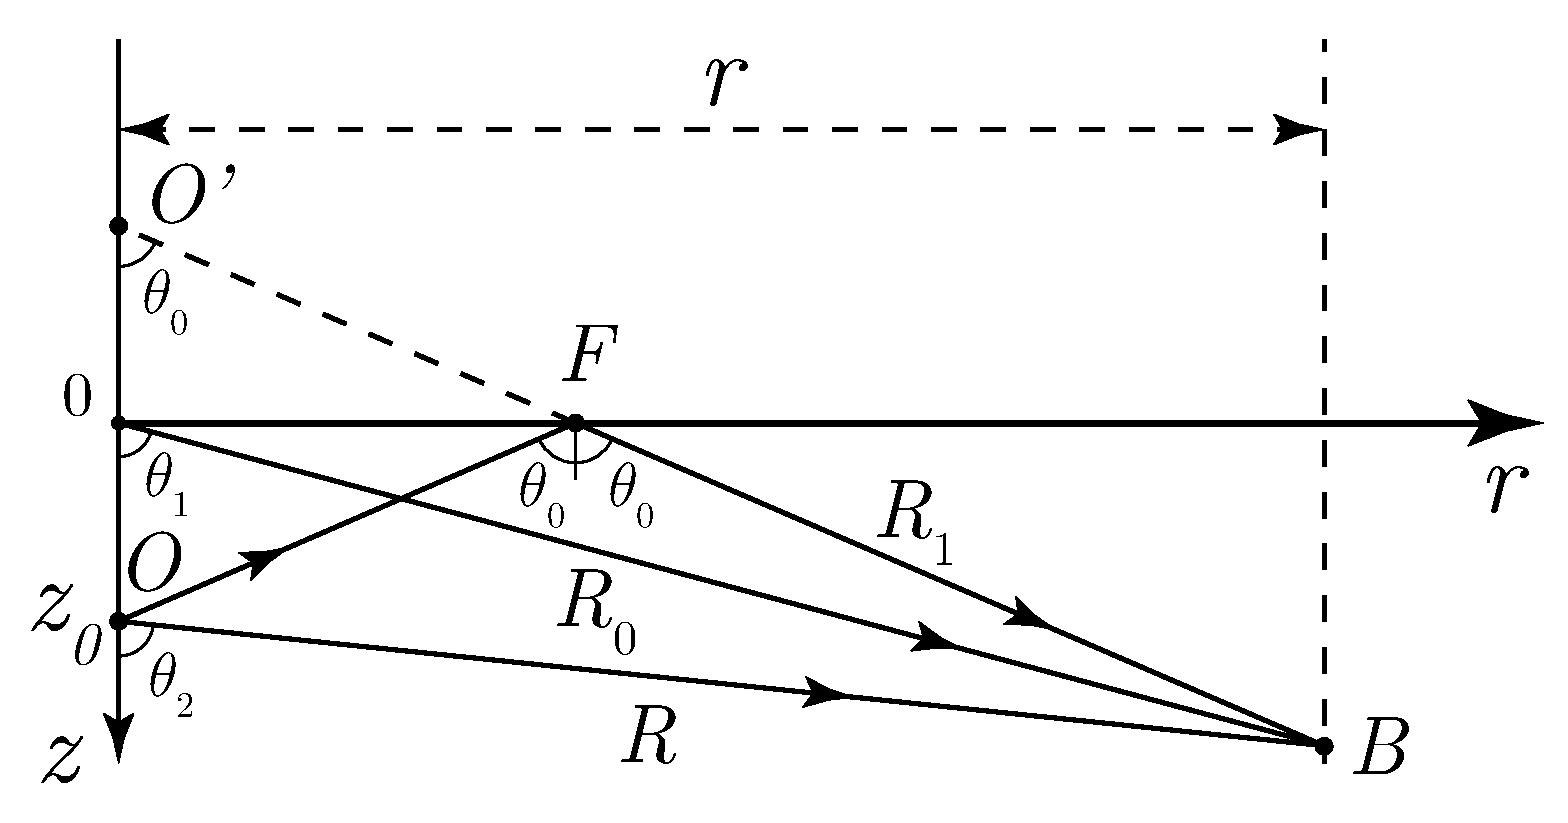
\includegraphics[width =0.6\linewidth]{fig/scheme.pdf}
	\caption{Расоложение излучателя $O$ и точки наблюдения $B$ по отношению к границе раздела}
	\label{fig:scheme}
\end{figure}
Поле мнимого источника соответствует полю, отраженному от границы раздела двух сред. Тогда для амплитуды суммарного давления запишем:
\begin{equation}
	P = \frac{e^{ikR}}{R}-\frac{e^{ikR_1}}{R_1}, \quad R^2 = r^2+(z-z_0)^2, \quad R_1^2 = r^2+(z+z_0)^2
	\label{eq:1}
\end{equation}
Модуль амплитуды давления в таком случае имеет вид:
\begin{equation}
	|P(h,R)| = \sqrt{ \frac{1}{R^2} + \frac{1}{R_1^2} - \frac{2}{R_1 R} \cos k \Delta R },\quad \Delta R = R-R_1,
	\label{eq:2}
\end{equation}
где $k$ - волновое число. При достаточно большом удалении ($R\gg z_0$), а также выполнении условия зоны Фраунгофера
$\frac{k z_0^2}{R_0}\ll 1$ можно свести выражения \eqref{eq:1} и \eqref{eq:2} к более простому виду:
\begin{equation}
	P = -\frac{2i}{R_0}\sin(k z_0 \cos \theta_1 )e^{ikR_0}
	\label{eq:3}
\end{equation}
\begin{equation}
	|P| = \frac{2}{R_0}|\sin (k z_0 \cos \theta_1)|
	\label{eq:4}
\end{equation}
Характеристика направленности системы из излучателя и поверхности воды имеет вид \eqref{eq:5}.
\begin{equation}
	\mathcal{F} = 2 |\sin(k z_0 \cos \theta_1)|
	\label{eq:5}
\end{equation}


\newpage
\section{Экспериментальная часть}
\paragraph{Описание установки}
Установка представляет собой устройство для излучения и приема акустических импульсов прямоугольной формы с ВЧ
заполнением, расположенные внутри бассейна с водой. Используется импульсный режим работы, так как при работе в
неприрывном режиме трудно разделить полезный и «мещающий» сигнал, многократно отраженный.

Длительность импульсов составляет $\tau \sim 100$ мкс (частота повторения $F\sim 100$ Гц), при этом должно
выполняться условие $\omega_c \tau \gg 1$, т.е. внутри импульса должно содержаться большое количество периодов
ВЧ-колебания, поэтому рабочая частота заполнения выбрана $f = 1$ МГц, длина волны в таком случае составляет $\lambda = 1.5$ мм.
\begin{figure}[h!]
	\centering
	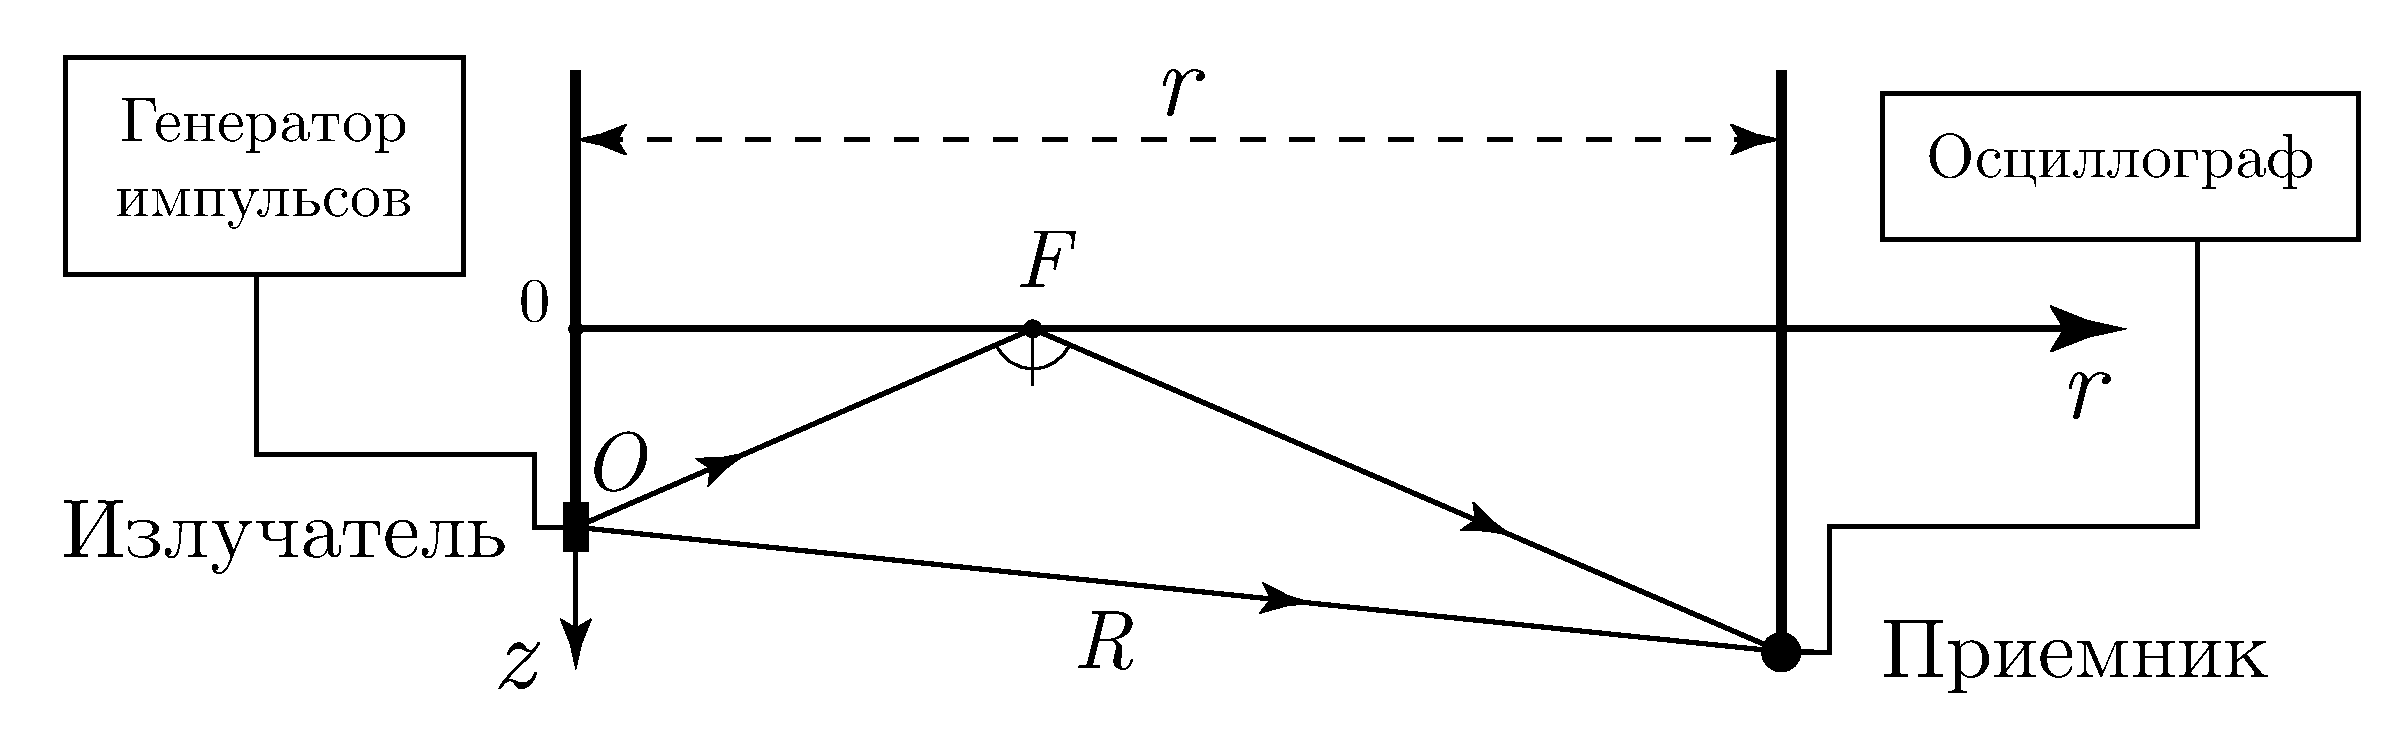
\includegraphics[width =0.7\linewidth]{fig/scheme0.pdf}
	\caption{Принципиальная схема установки}

\end{figure}
\subsection{Диаграмма направленности излучателя}
Для снятия диаграммы направленности, излучатель был погружен в воду на глубину 15 см. Приемный щуп был расположен на той
же глубине, а расстояние от приемника определялось несколькими условиями.

Первое - проведение измерений в зоне Фраунгофера, для того, чтобы вести работу с сформировавшимся фронтом волны. Условие
выглядит следующим образом:
\begin{equation}
	L > \frac{2D^2}{\lambda} \Rightarrow L > \frac{2 \cdot 10^{-4}}{1.5 \cdot 10^{-3}} \simeq 0.13 \text{ м} 
	\label{eq:exp:fraungofer}
\end{equation}
где $L$ - расстояние между источником и приемником, $D$ - характерный размер источника(10 мм), $\lambda$ - длина волны
излучения ( $f = 1$ МГц, $\lambda = 1.5$ мм). 

Второе - прямой и отраженный импульс должны полностью разделяться по времени прихода. Чтобы это условие выполнялось,
необходимо, чтобы время прихода отраженного импульса $t_2$ было больше, чем величина $t_1+\tau$, где $t_1$ - время
прихода прямого импульса, а $\tau$ - длительность импульса.
\begin{figure}[h!]
	\centering
	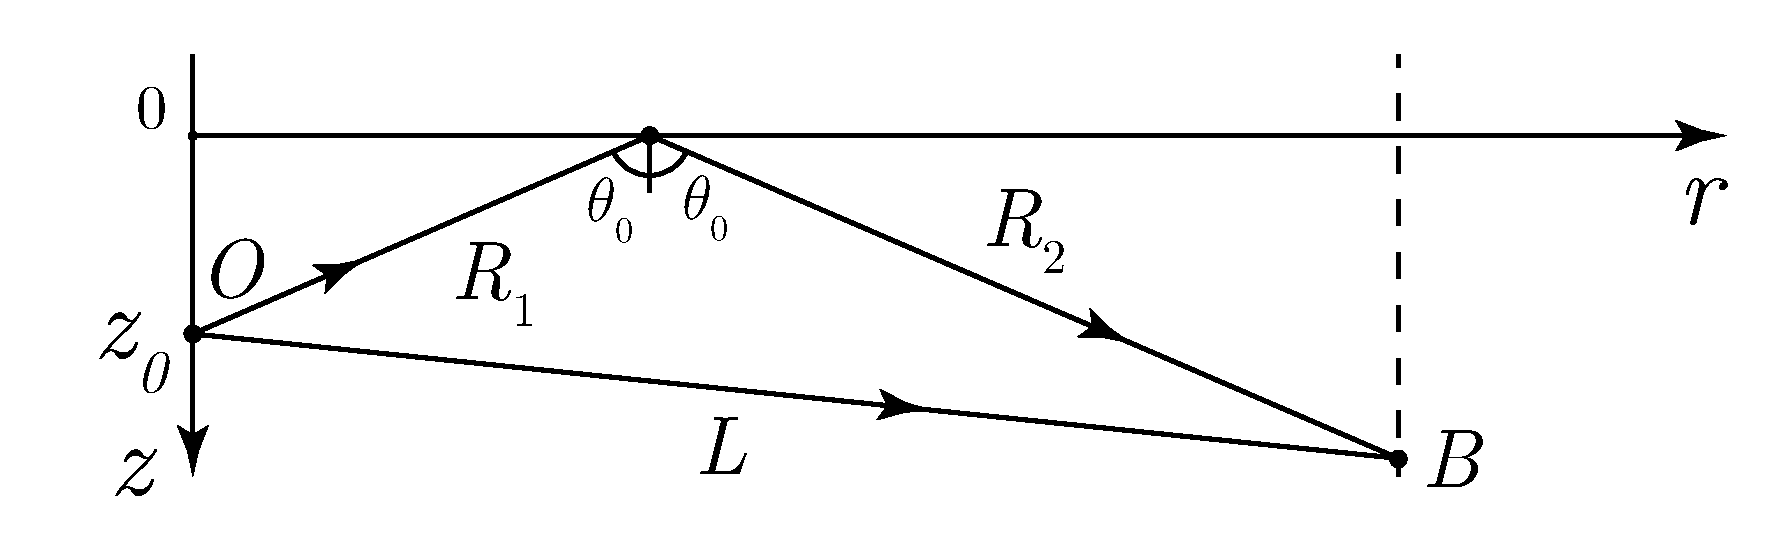
\includegraphics[width =0.7\linewidth]{fig/scheme2.pdf}
	\caption{Схема к рассчету расстояния меджу источником и приемником}
	\label{fig:expt:scheme2}
\end{figure}

\begin{equation}
	t_2 > t_1 + \tau, \quad t_1 = \frac{L}{c}, t_2 = \frac{R_1+R_2}{c}
\end{equation}
В достаточно грубом приближении, считая $L \sim 1$ м, а $R_1+R_2 \sim 1.5$ м, можно получить:
\begin{equation}
	\tau < \frac{R_1+R_2-L}{c} \simeq \frac{0.5}{1500} = 3 \cdot 10^{-4} \text{ с}
\end{equation}
\begin{equation}
	\tau < 300 \text{ мкс}
	\label{eq:time_cond}
\end{equation}
В работе использовалось $\tau = 100$ мкс, что удовлетворяет условию \eqref{eq:time_cond}.

Отнормированная диаграмма направленности излучателя, а также расчитанная теоретически в приближении плоского диска
приведены на рис. \ref{fig:direct}. В качестве теоретической характеристики использовалась характеристика круглой
плоской антенны с диаметром $d$:
\begin{equation}
	b(\theta) = \frac{2 J_1[ \frac{\pi d}{\lambda} \cos \theta ]}{\frac{\pi d}{\lambda} \cos \theta },
	\label{eq:bessel_disk}
\end{equation}
где $J_1$ - функция Бесселя первого порядка. Отметим, что аргумент $\theta$ был смещен на $\frac{\pi}{2}$, так как в
таком виде функция Бесселя правильнее описывает диаграмму направленности. Такое смещени можно делать, так как ноль по
значению угла выбирался нами произвольно, и может не совпадать с тем, как выбирался ноль при выводе уравнения \eqref{eq:bessel_disk}. 
\begin{figure}[h!]
	\centering
	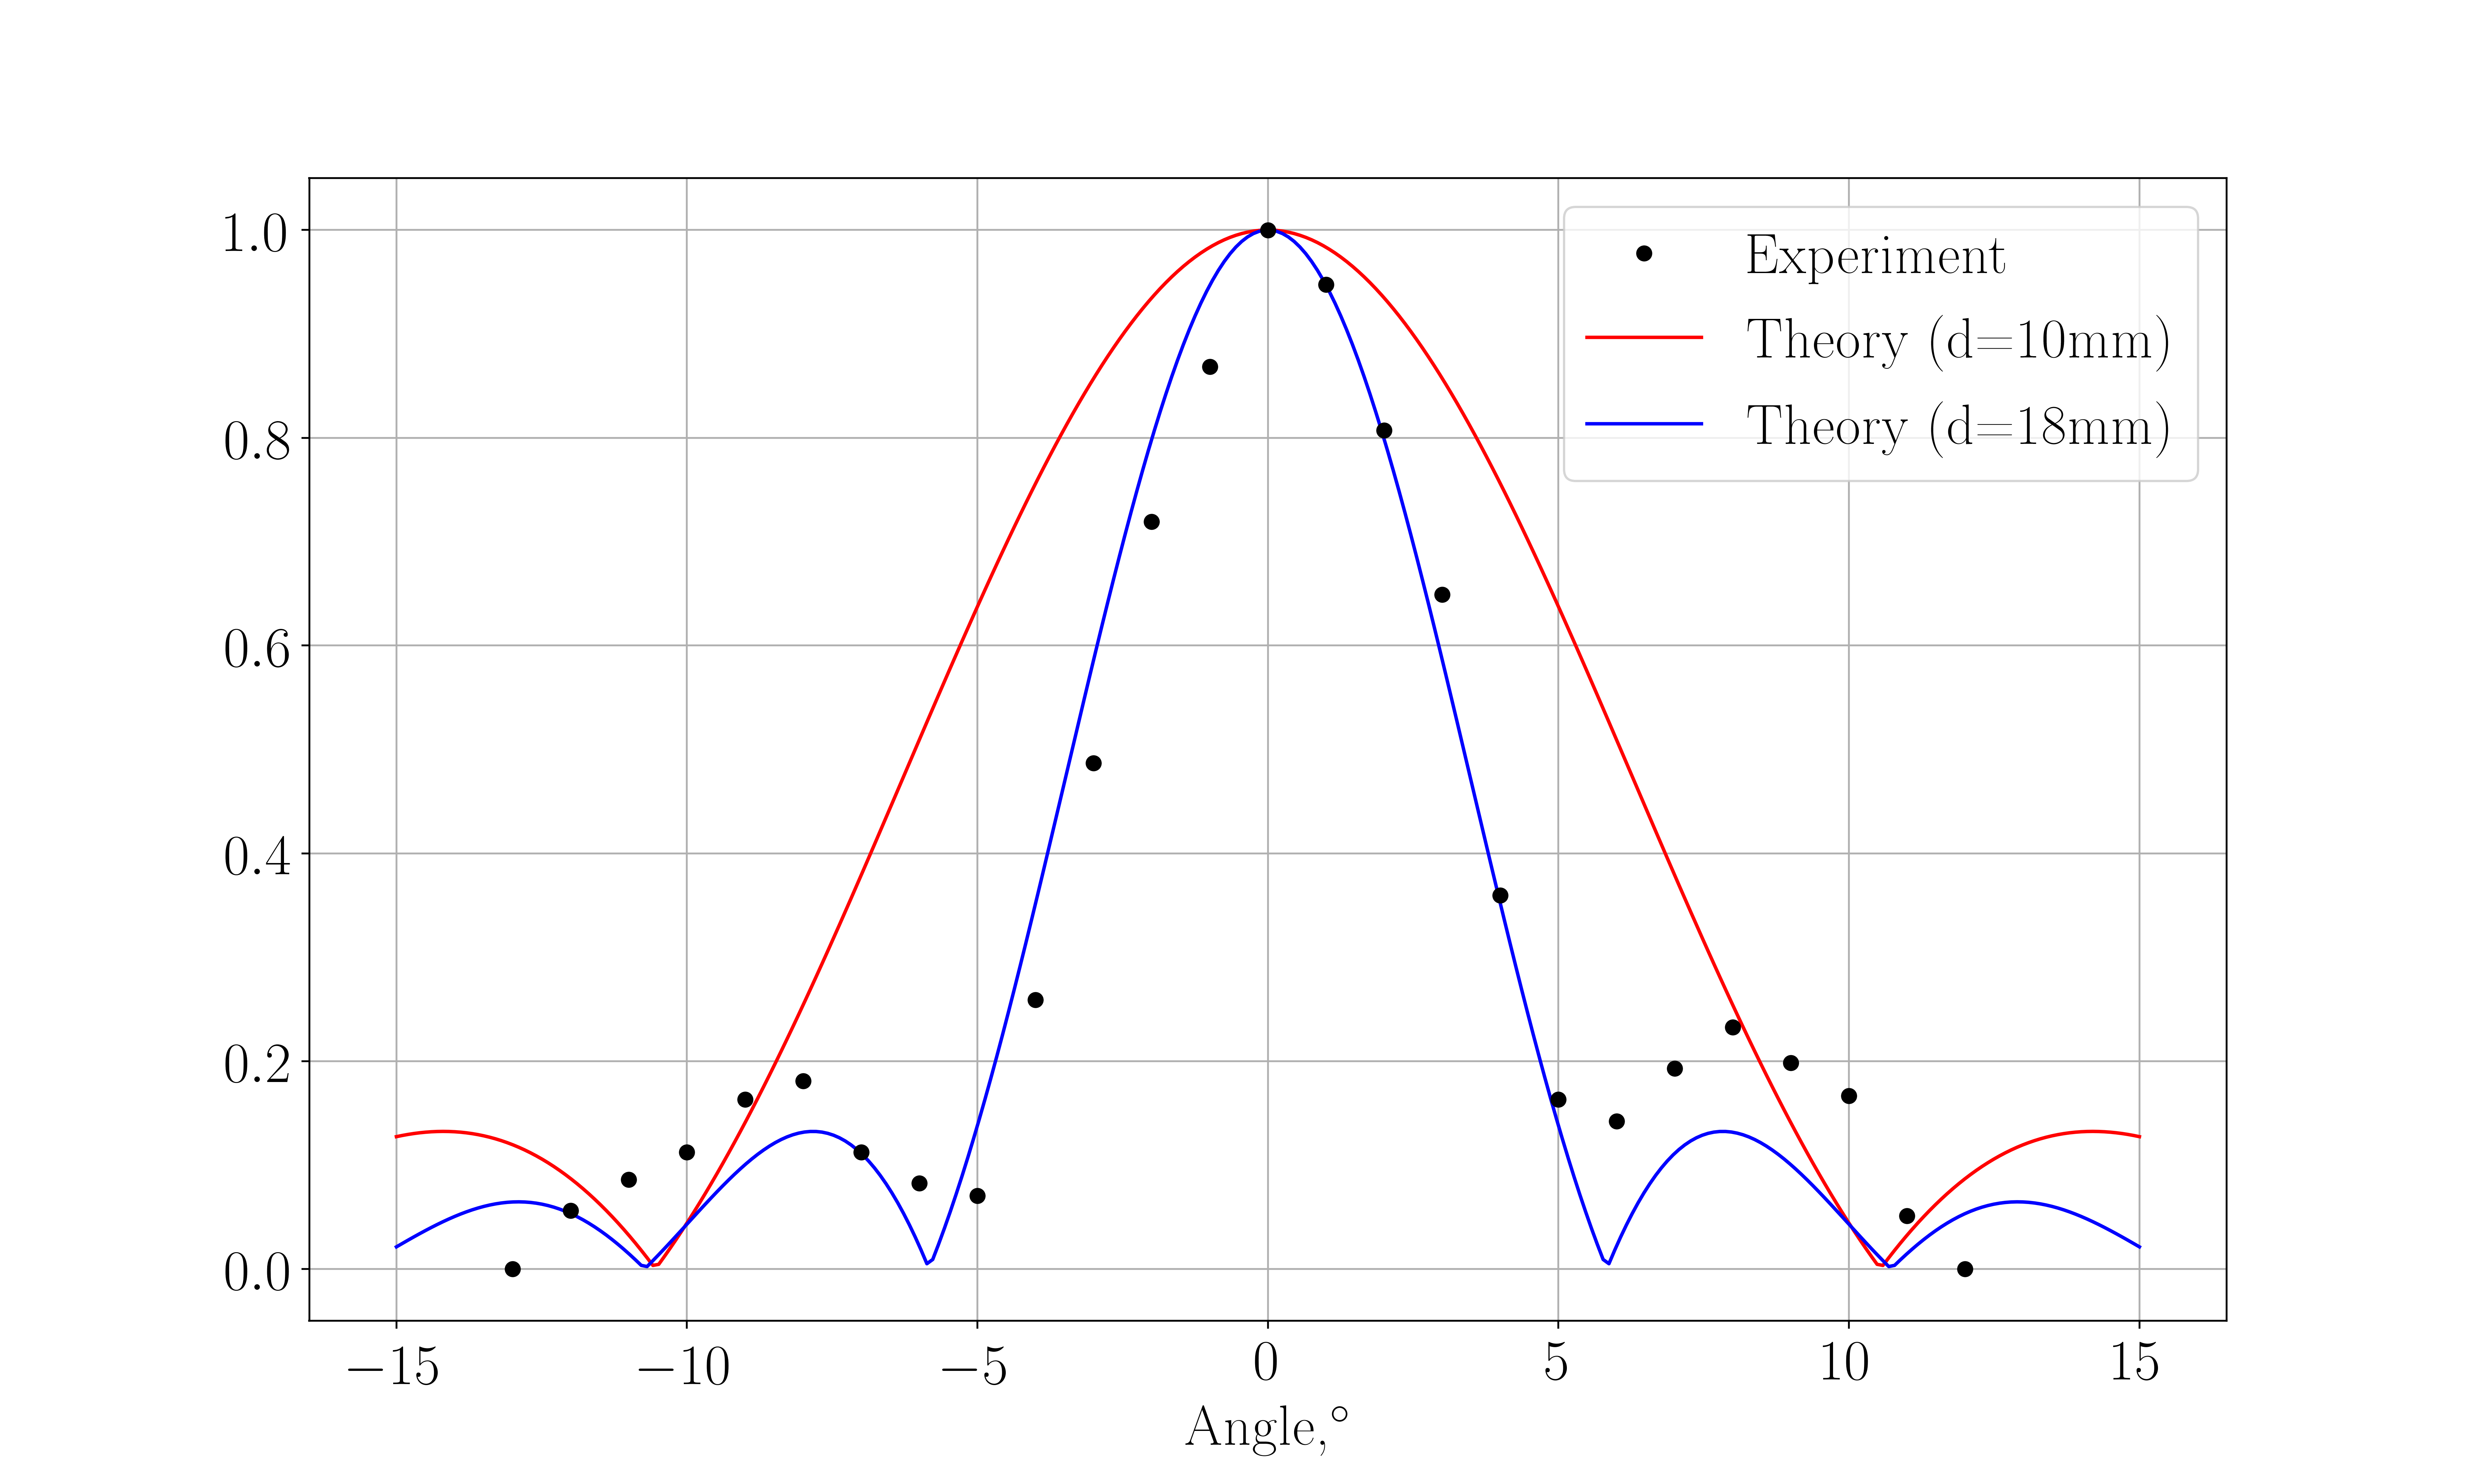
\includegraphics[width=0.9\linewidth]{fig/direct.png}
	\caption{Нормированная диаграммма направленности излучателя, и теоретическая характеристика для плоского диска диаметром $d$}
	\label{fig:direct}
\end{figure}

Экспериментальная зависимость достаточно хорошо описывается приближением для плоского диска, однако имеет некоторую
степень несимметричности, что нормально для реальных излучателей.
Определенный эффективный диаметр излучателя составляет $d = 18$ мм.
\subsection{Исследование распределения звукового давления}
\begin{figure}[h!]
	\centering
	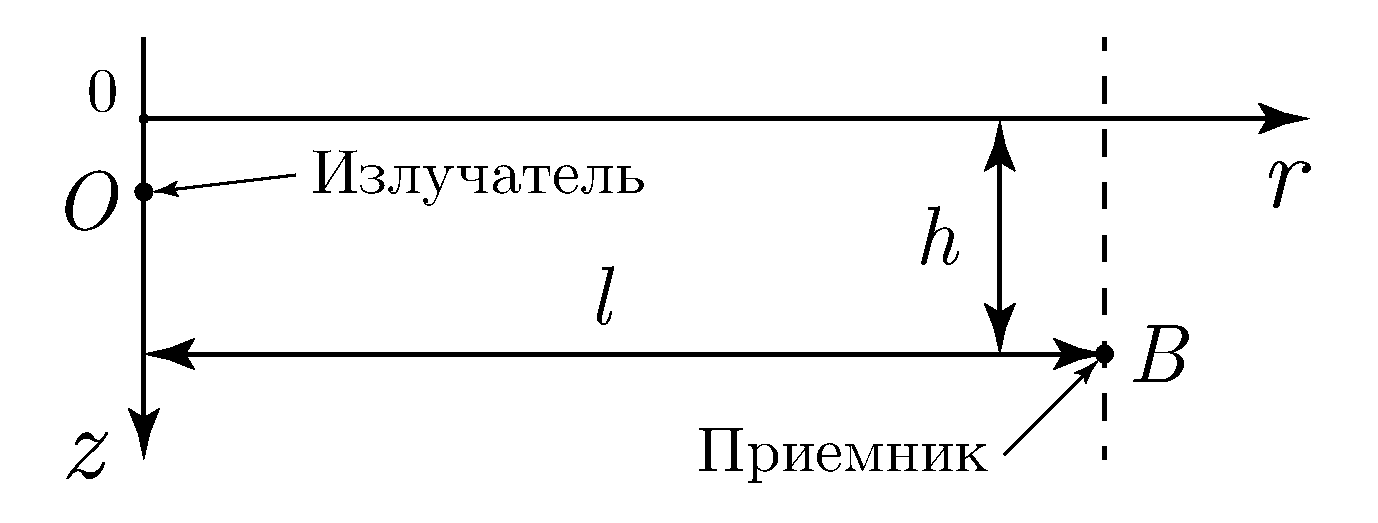
\includegraphics[width =0.5\linewidth]{fig/scheme3.pdf}
	\caption{Схема постановки эксперимента}
	\label{fig:expt:scheme3}
\end{figure}
Излучатель был расположен на глубине $\sim 3-4$ см, чтобы полностью быть погруженным в воду.
С помощью приемного щупа было произведено исследовано распределение звукового давления в ванне, были произведены три
продольных разреза на глубинах $h = 1,2.5,4$ см, и три вертикальных среза на расстояниях $l=70,100,130$ см.

Теоретическое значение для модуля амплитуды суммарного давления рассчитывалось по формуле \eqref{eq:pressure}:
\begin{equation}
	|P(h,R)| = \sqrt{ \frac{1}{R^2} + \frac{1}{R_1^2} - \frac{2}{R_1 R} \cos k \Delta R },\quad \Delta R = R-R_1,
	\label{eq:pressure}
\end{equation}
где $R^2 = l^2+(h-z_0)^2$, а $R_1^2 = l^2 + (h+z_0)^2$, $k$ - волновое число. Также использовалась
приближенная формула \eqref{eq:app_pressure} (приведена на рис. \ref{fig:task22}), однако использовалась только один
раз, для сравнения, так как практически не отличается от \eqref{eq:pressure}.
\begin{equation}
	|P| = \frac{2}{R_0}|\sin ( k z_0 \cos \theta_1 )|
	\label{eq:app_pressure}
\end{equation}

Амплитуды максимумов и минимумов для продольных срезов приведены на рис. \ref{fig:task21}, \ref{fig:task22}, \ref{fig:task23}. По
снятым экспериментальным данным была определена глубина погружения эффективного центра излучателя $z_0 \in [3.25, 4.2]$
см.

\begin{figure}[h!]
	\centering
	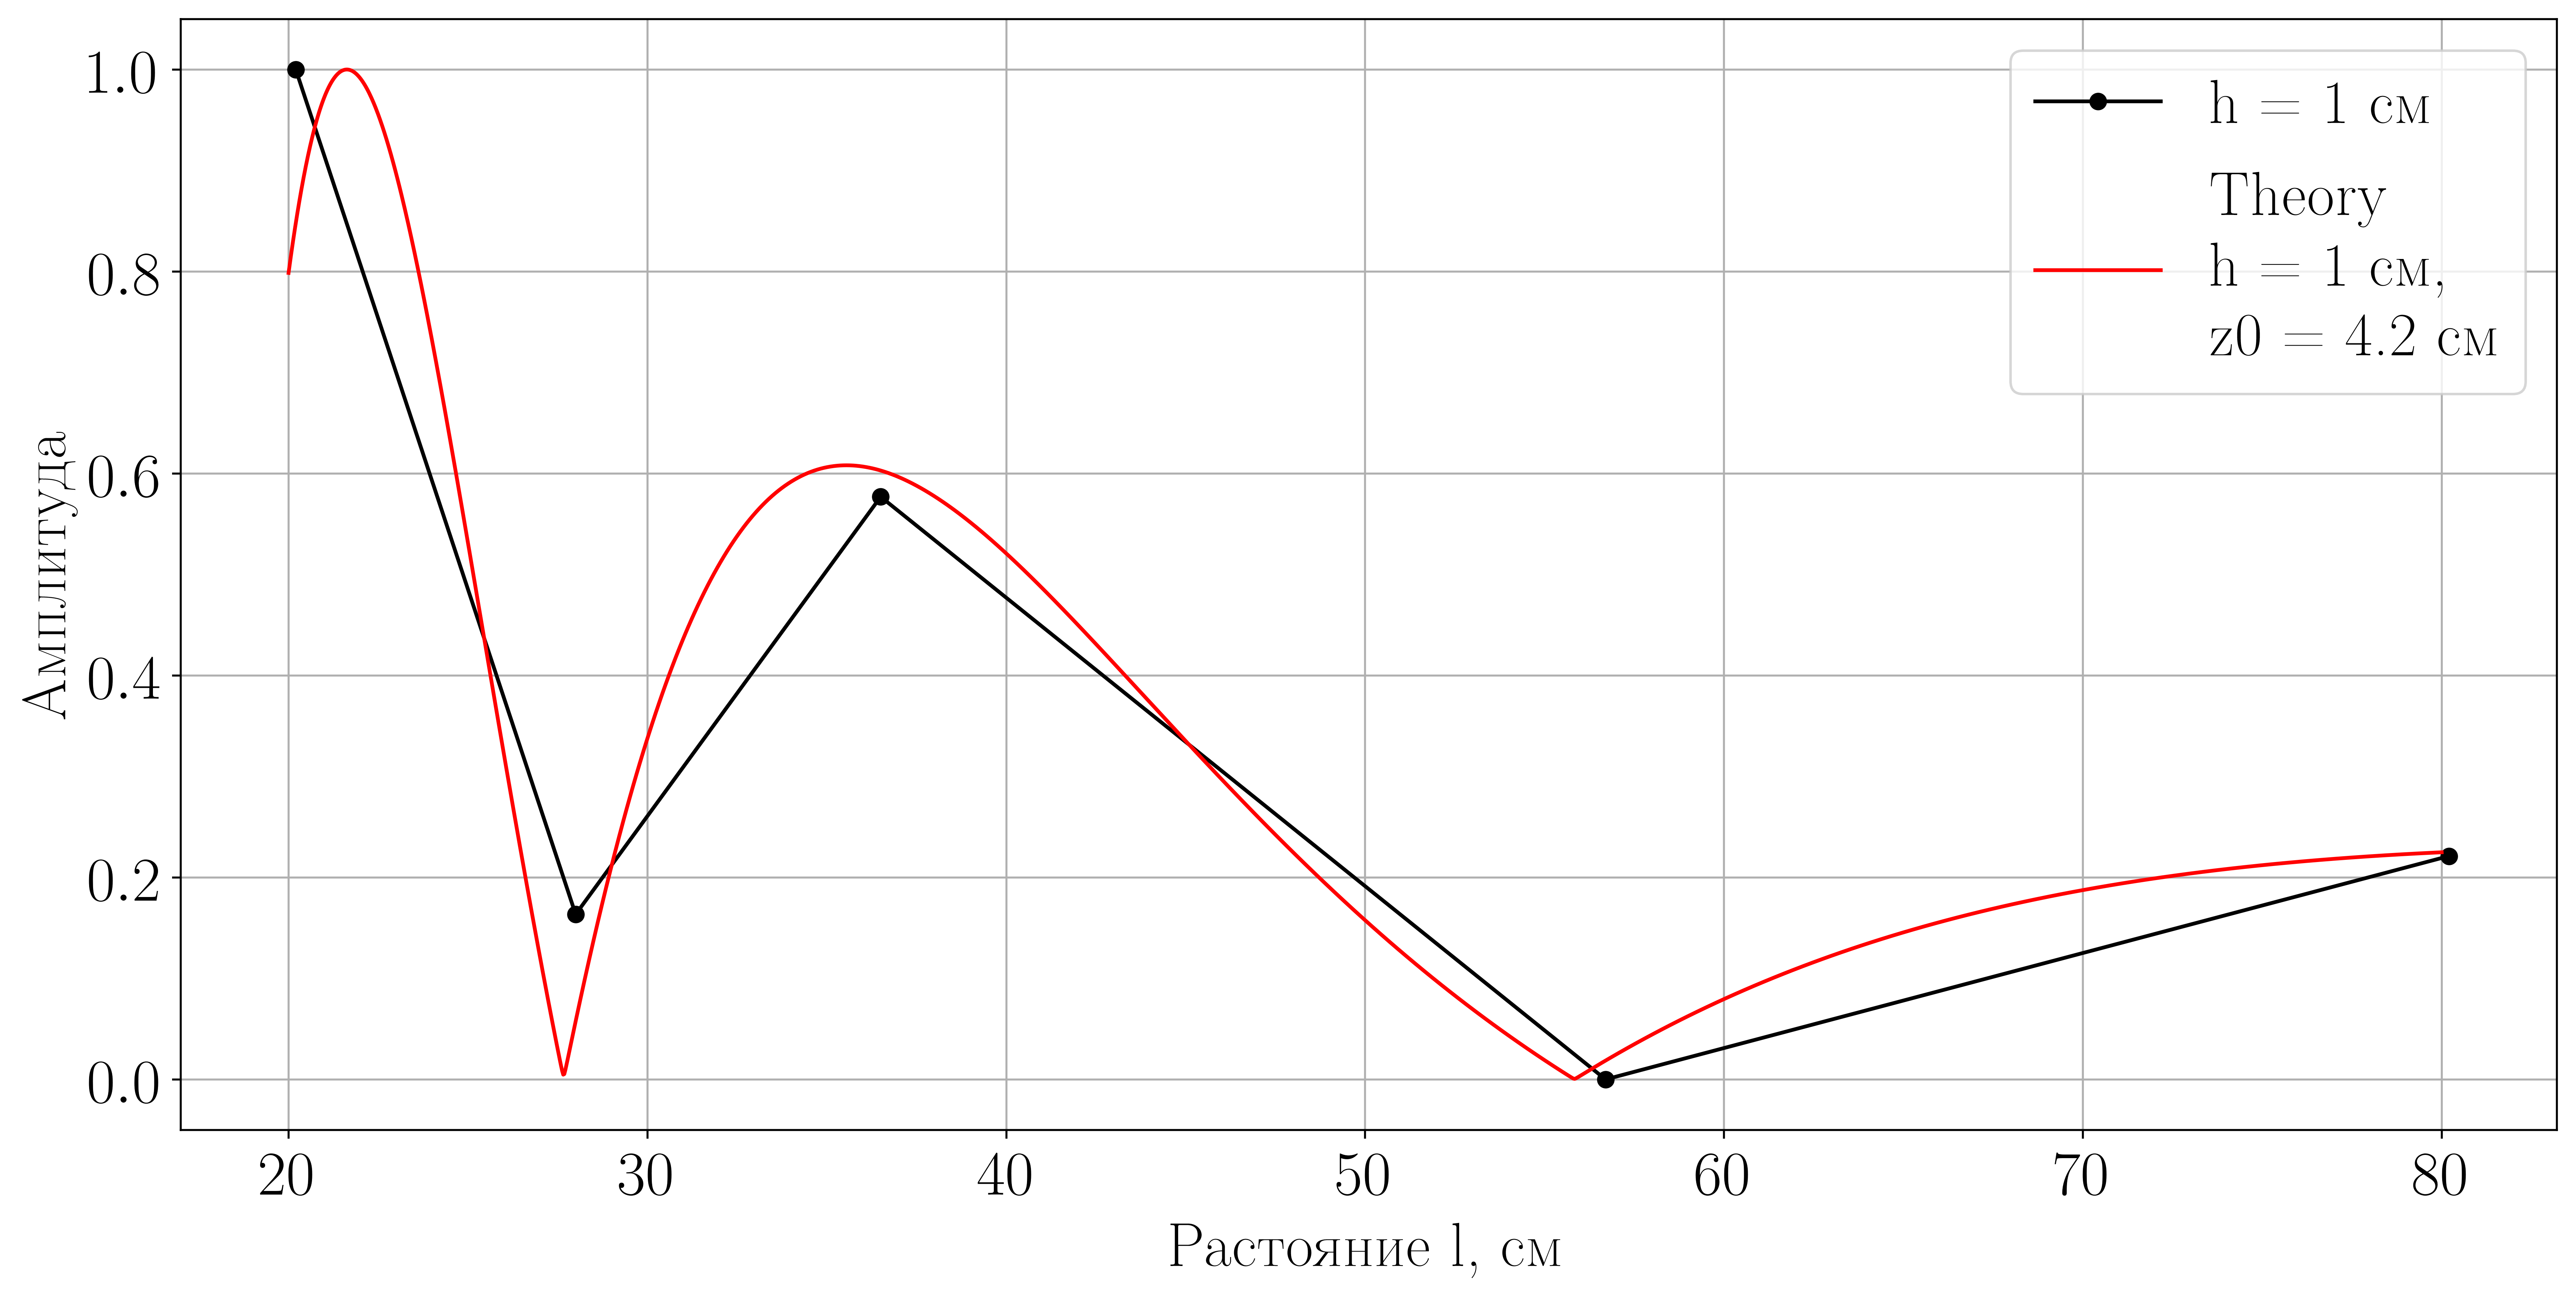
\includegraphics[width =0.79\linewidth]{fig/task21}
	\caption{Амплитуды максимумов и минимумов при продольном срезе, на глубине $h=1$ см}
	\label{fig:task21}
\end{figure}
\begin{figure}[h!]
	\centering
	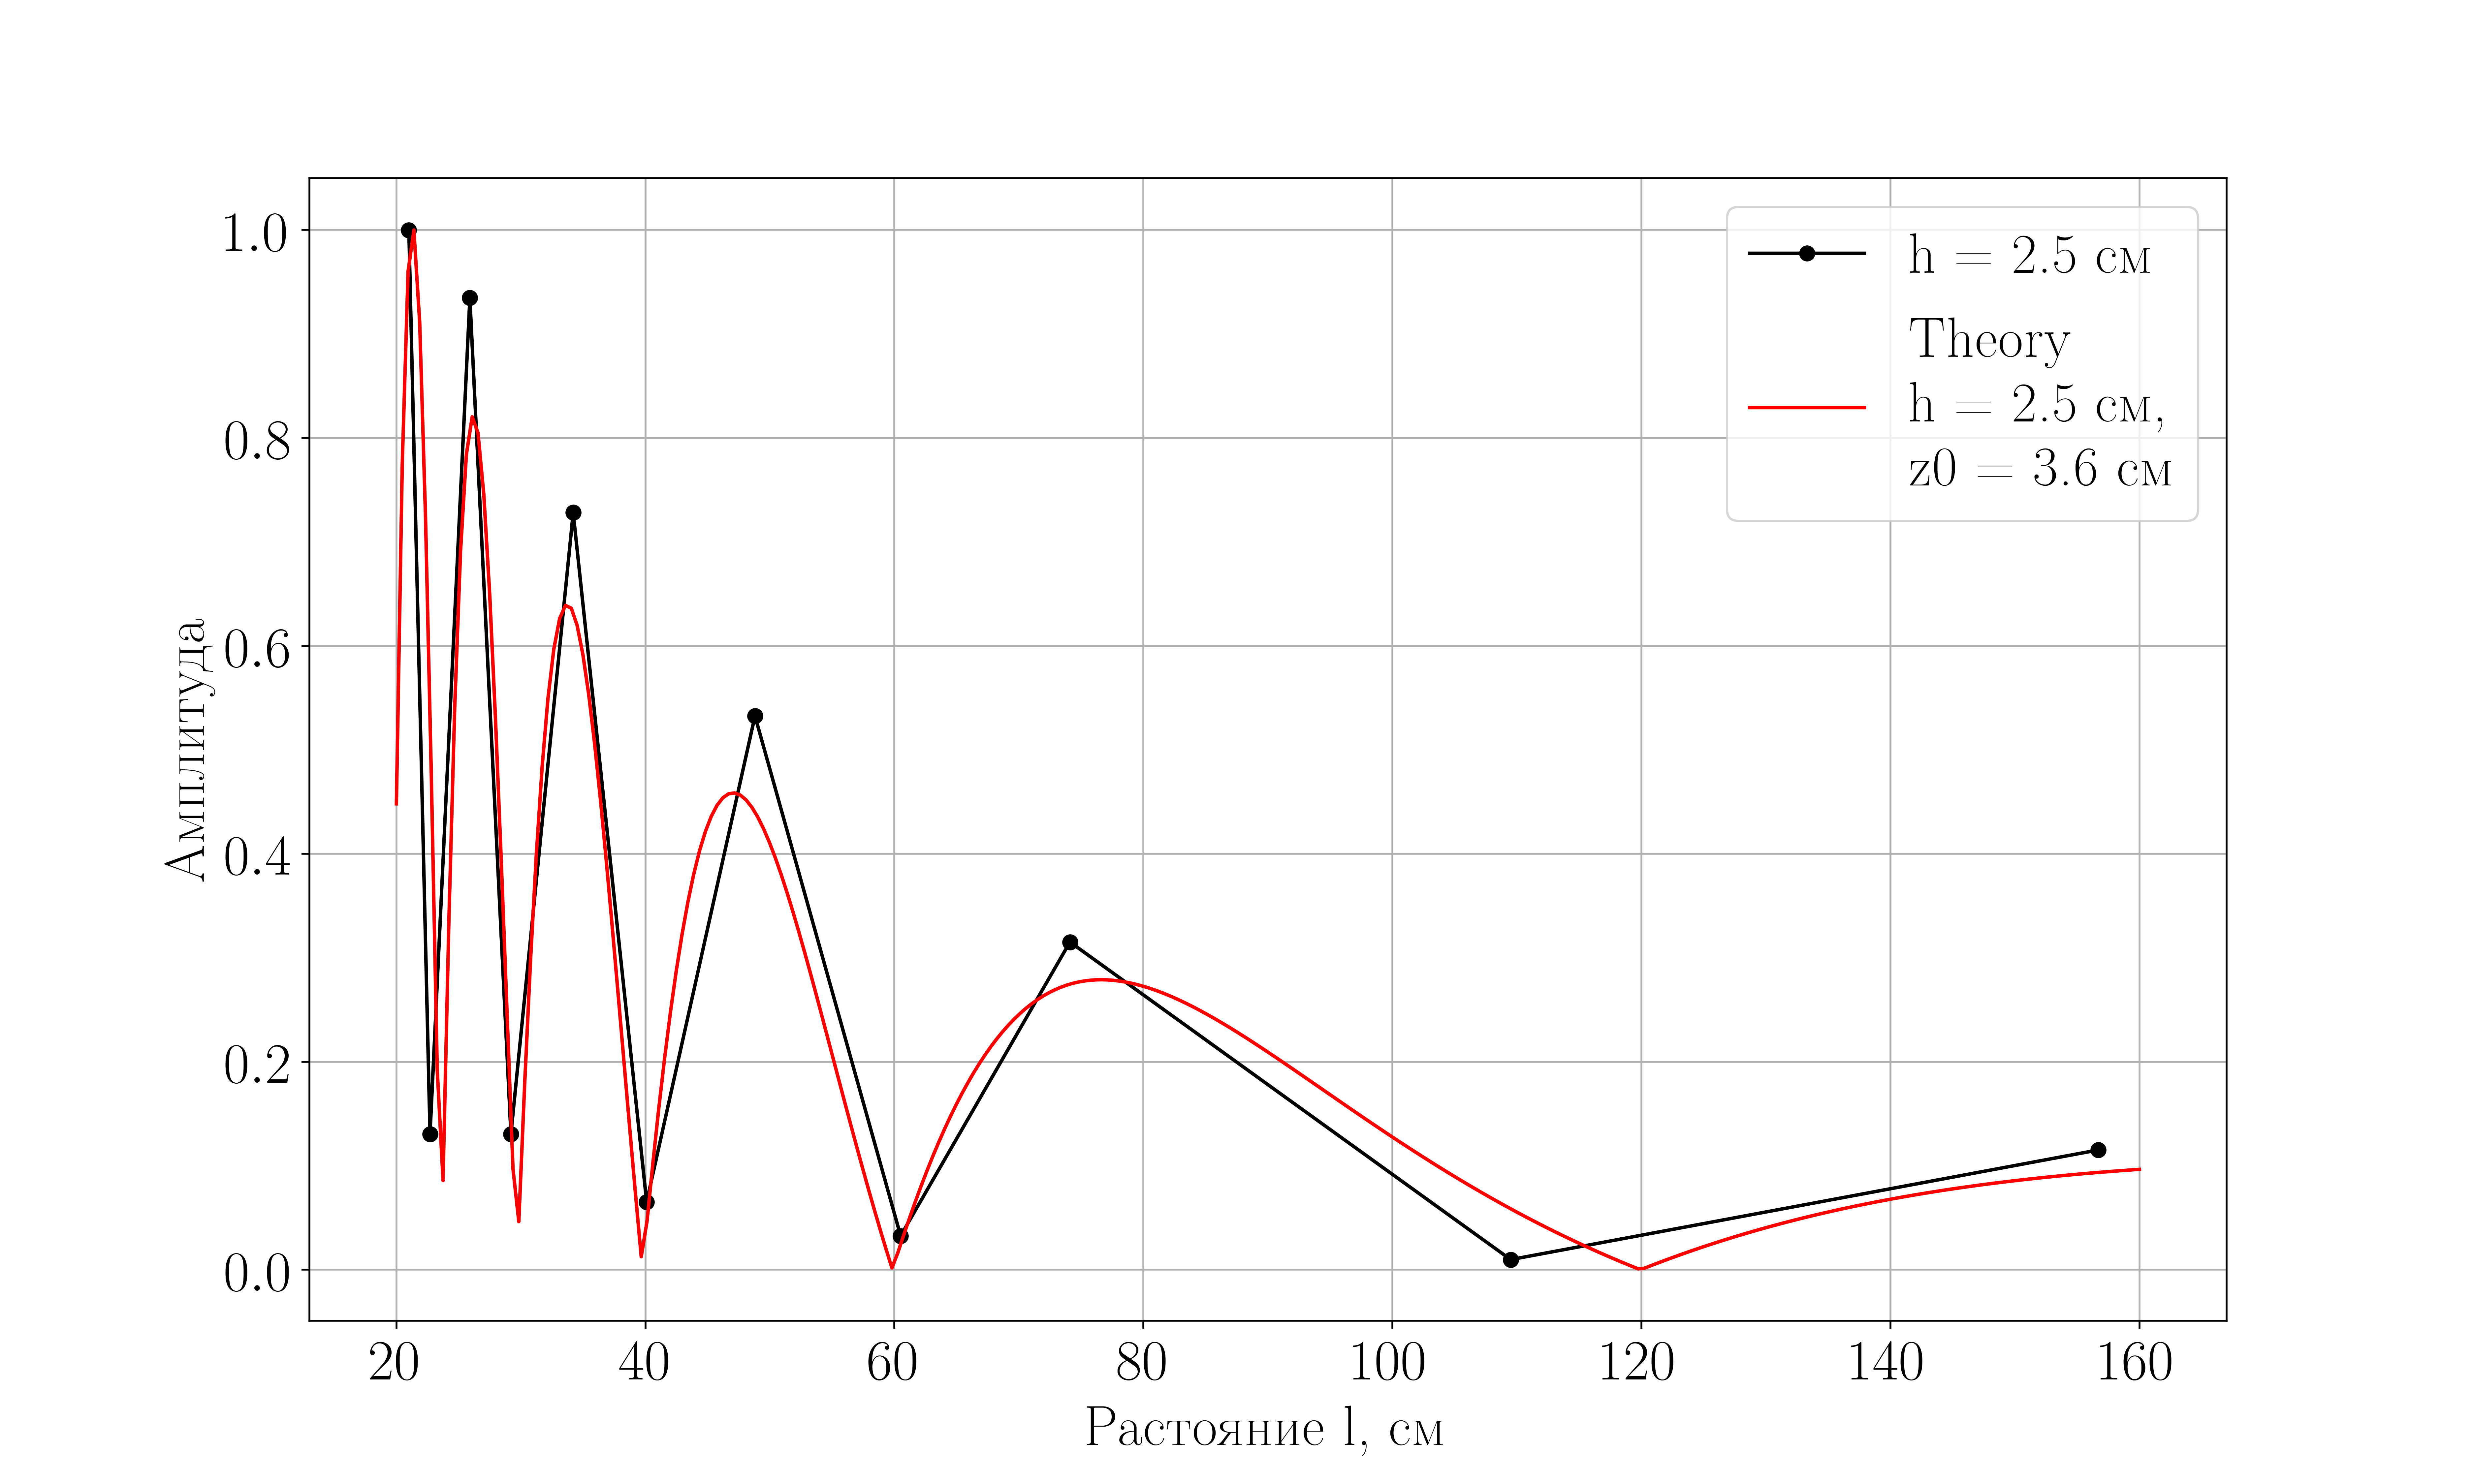
\includegraphics[width =0.79\linewidth]{fig/task22}
	\caption{Амплитуды при продольном срезе, на глубине $h=2.5$ см}
	\label{fig:task22}
\end{figure}
\begin{figure}[h!]
	\centering
	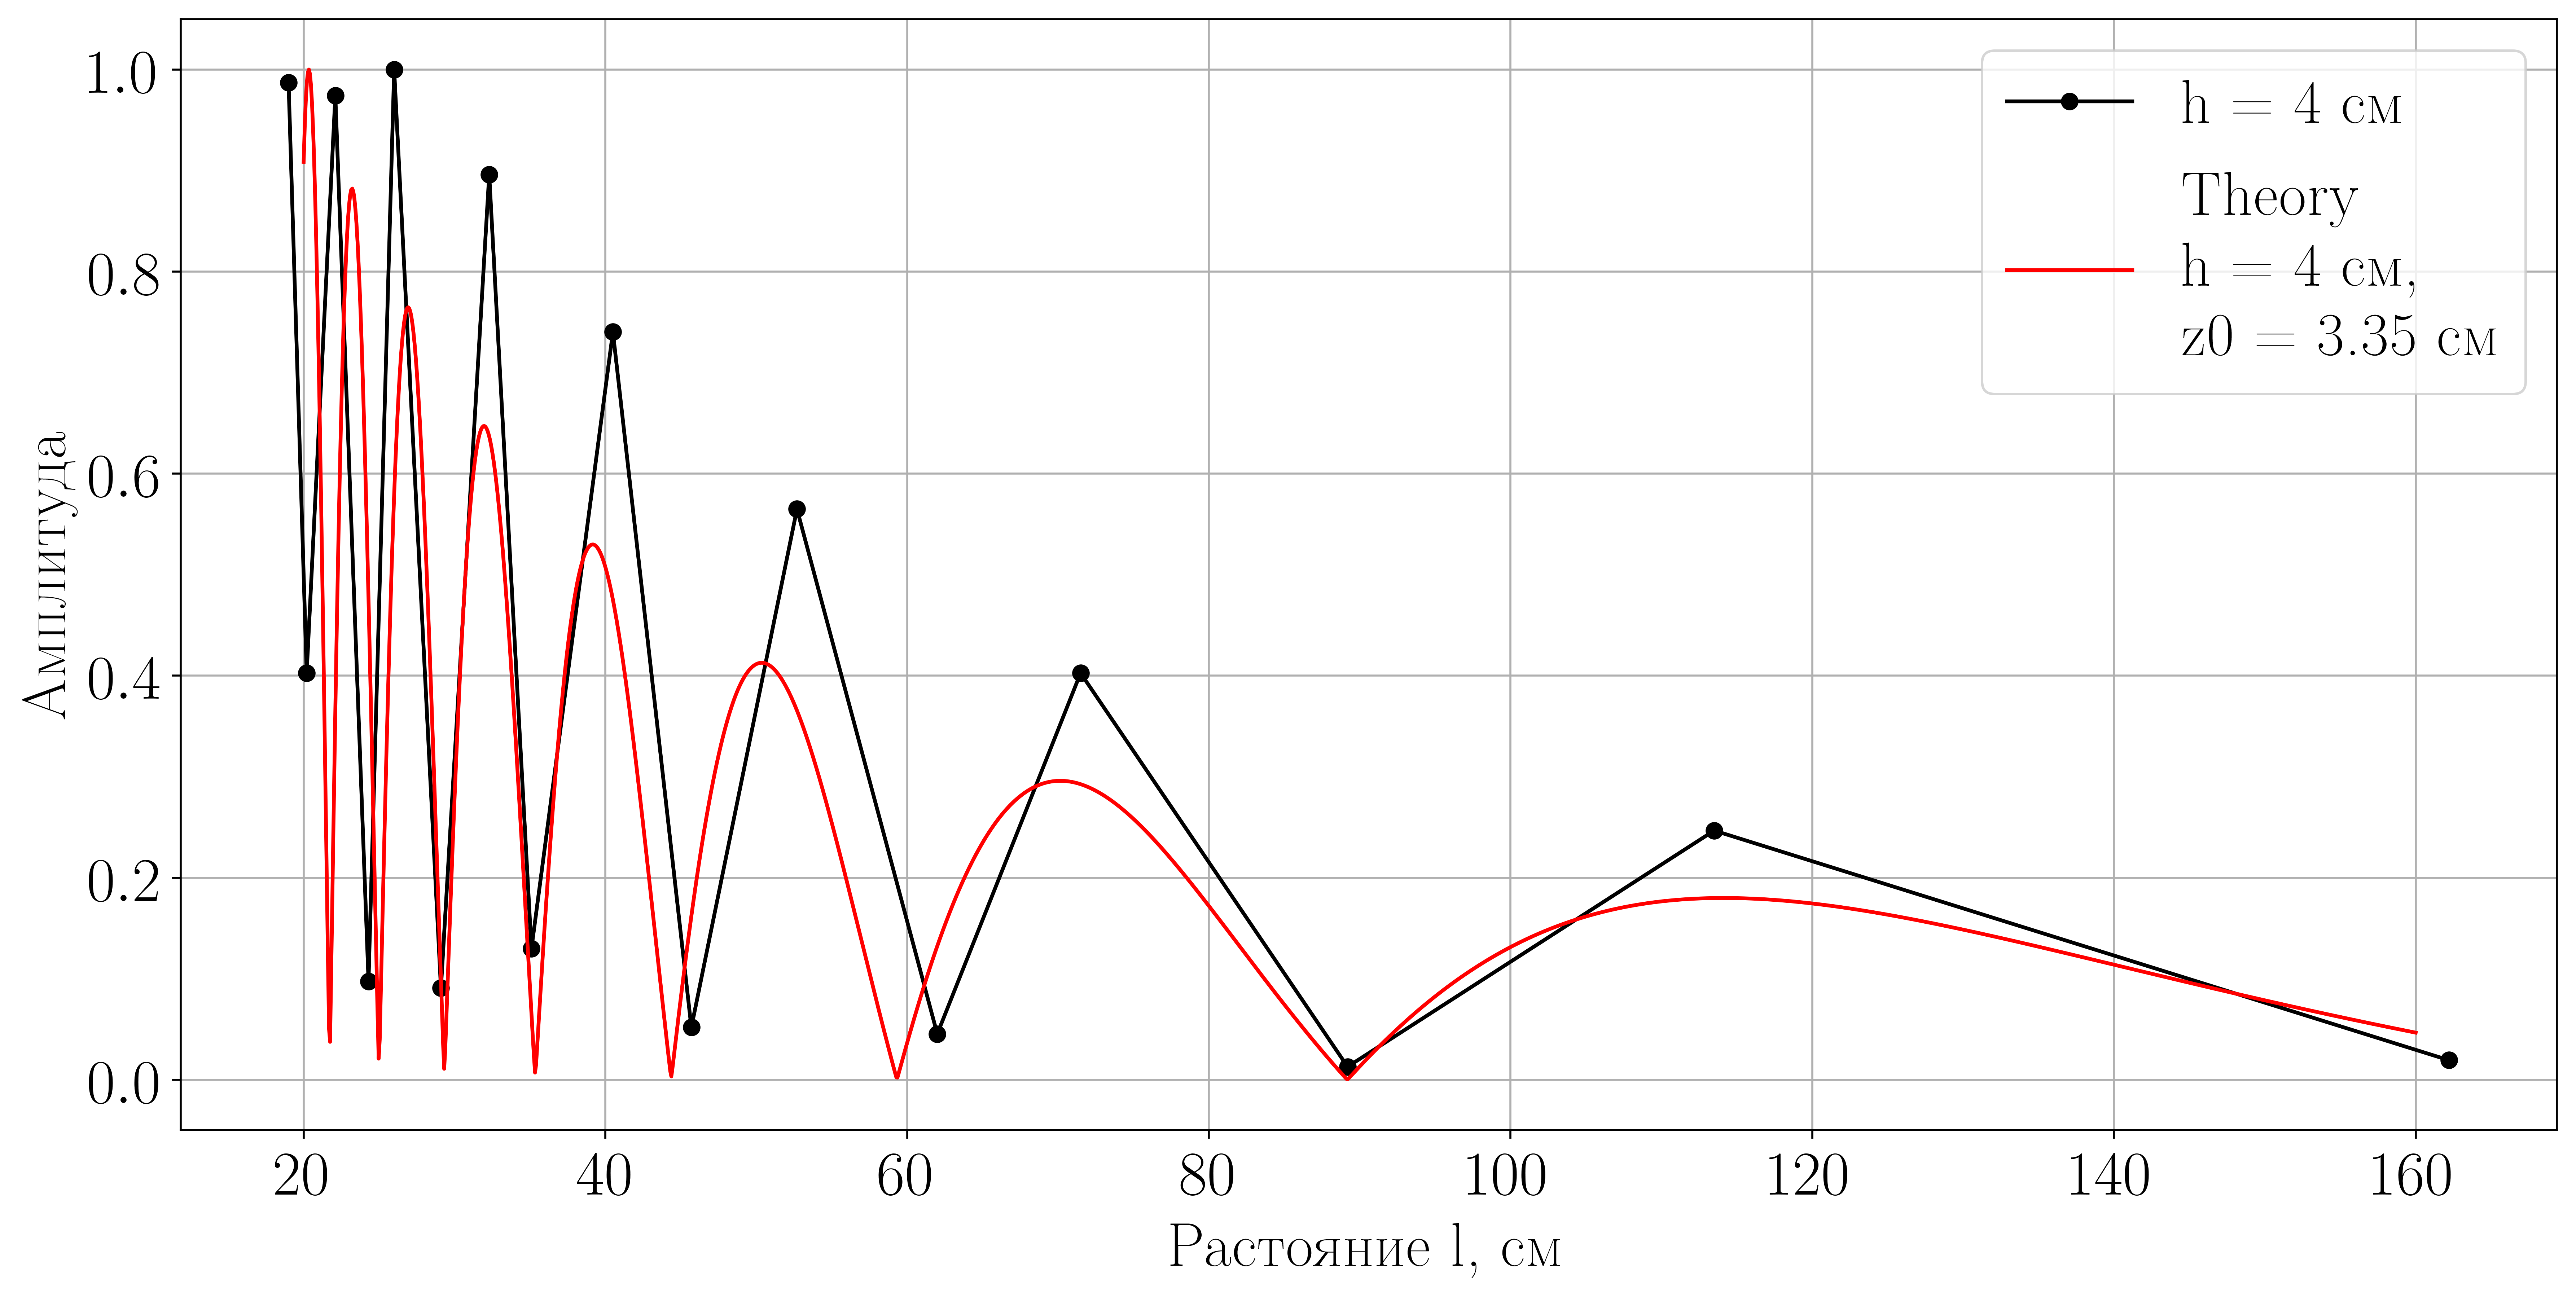
\includegraphics[width =0.79\linewidth]{fig/task23}
	\caption{Амплитуды при продольном срезе, на глубине $h=4$ см}
	\label{fig:task23}
\end{figure}

В целом наблюдается достаточное хорошее совпадение эксперимента с теорией. В местах, где амплитуда минимумов не равна
нулю, преимущестсвенно играют роль шумы. Не совпадение по абсолютным значением можно объяснить нормировкой, и тем
фактом, что непосредственно измеряемой в эксперименте величной была амплитуда напряжения, а в теории рассчитывается
амплитуда давления. 


\begin{figure}[h!]
	\centering
	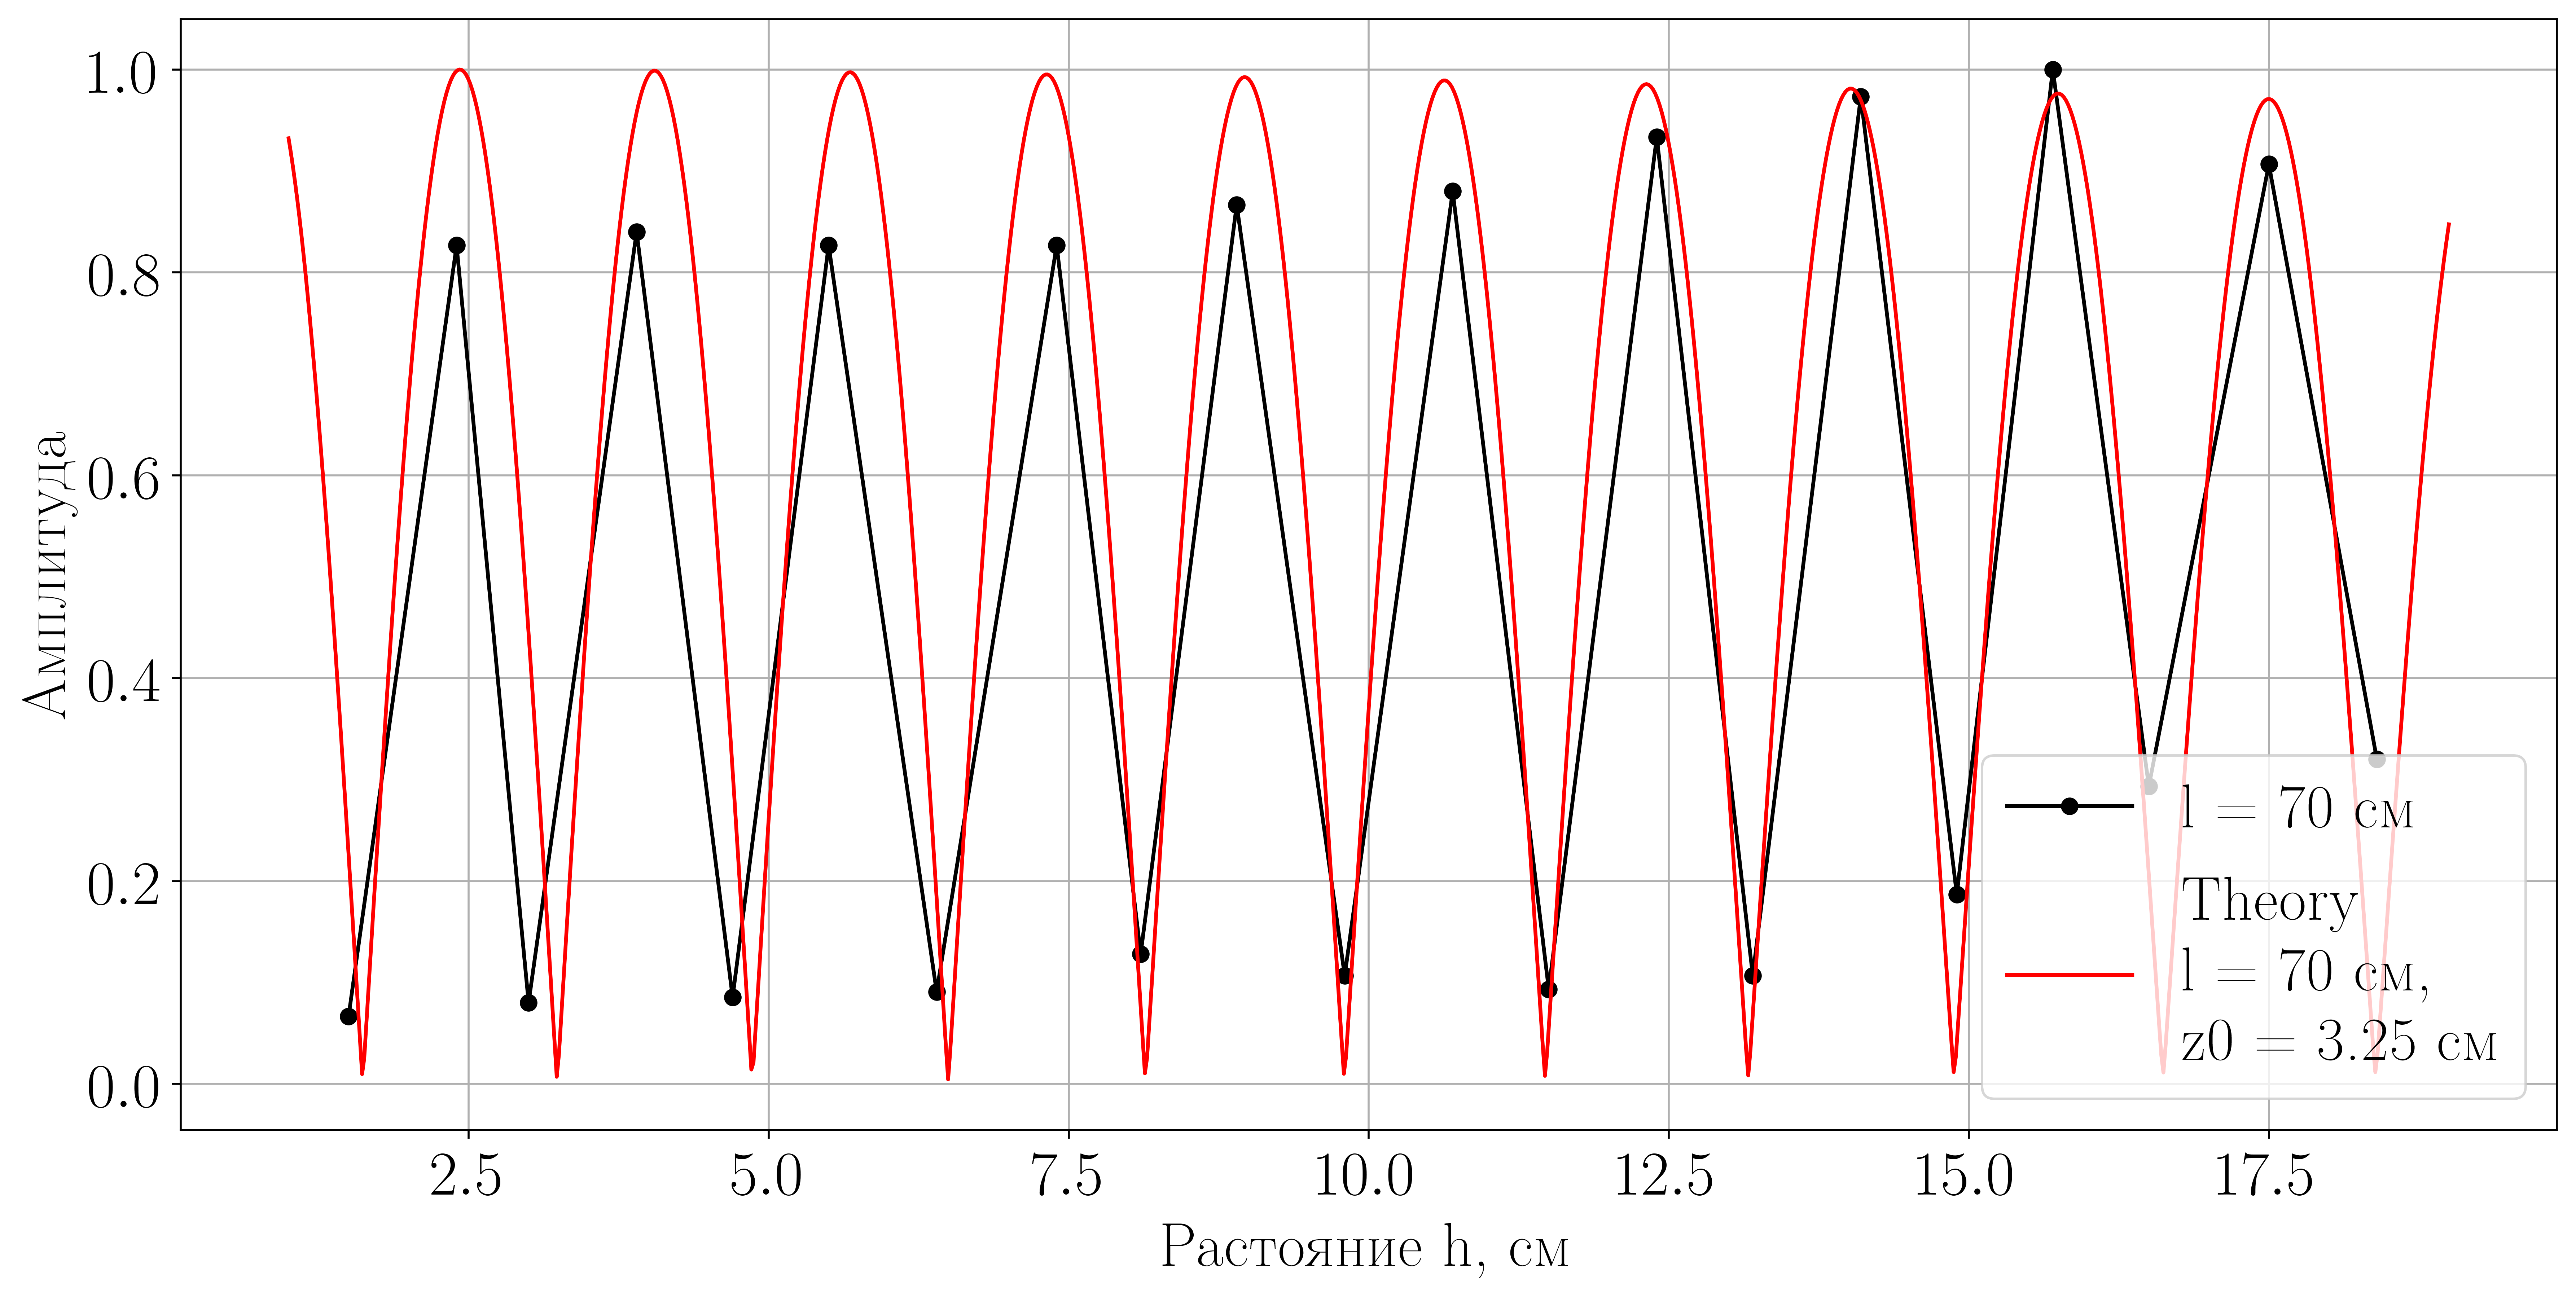
\includegraphics[width =0.79\linewidth]{fig/task31}
	\caption{Амплитуды при вертикальном срезе, на расстоянии $l=70$ см}
	\label{fig:task31}
\end{figure}

\begin{figure}[h!]
	\centering
	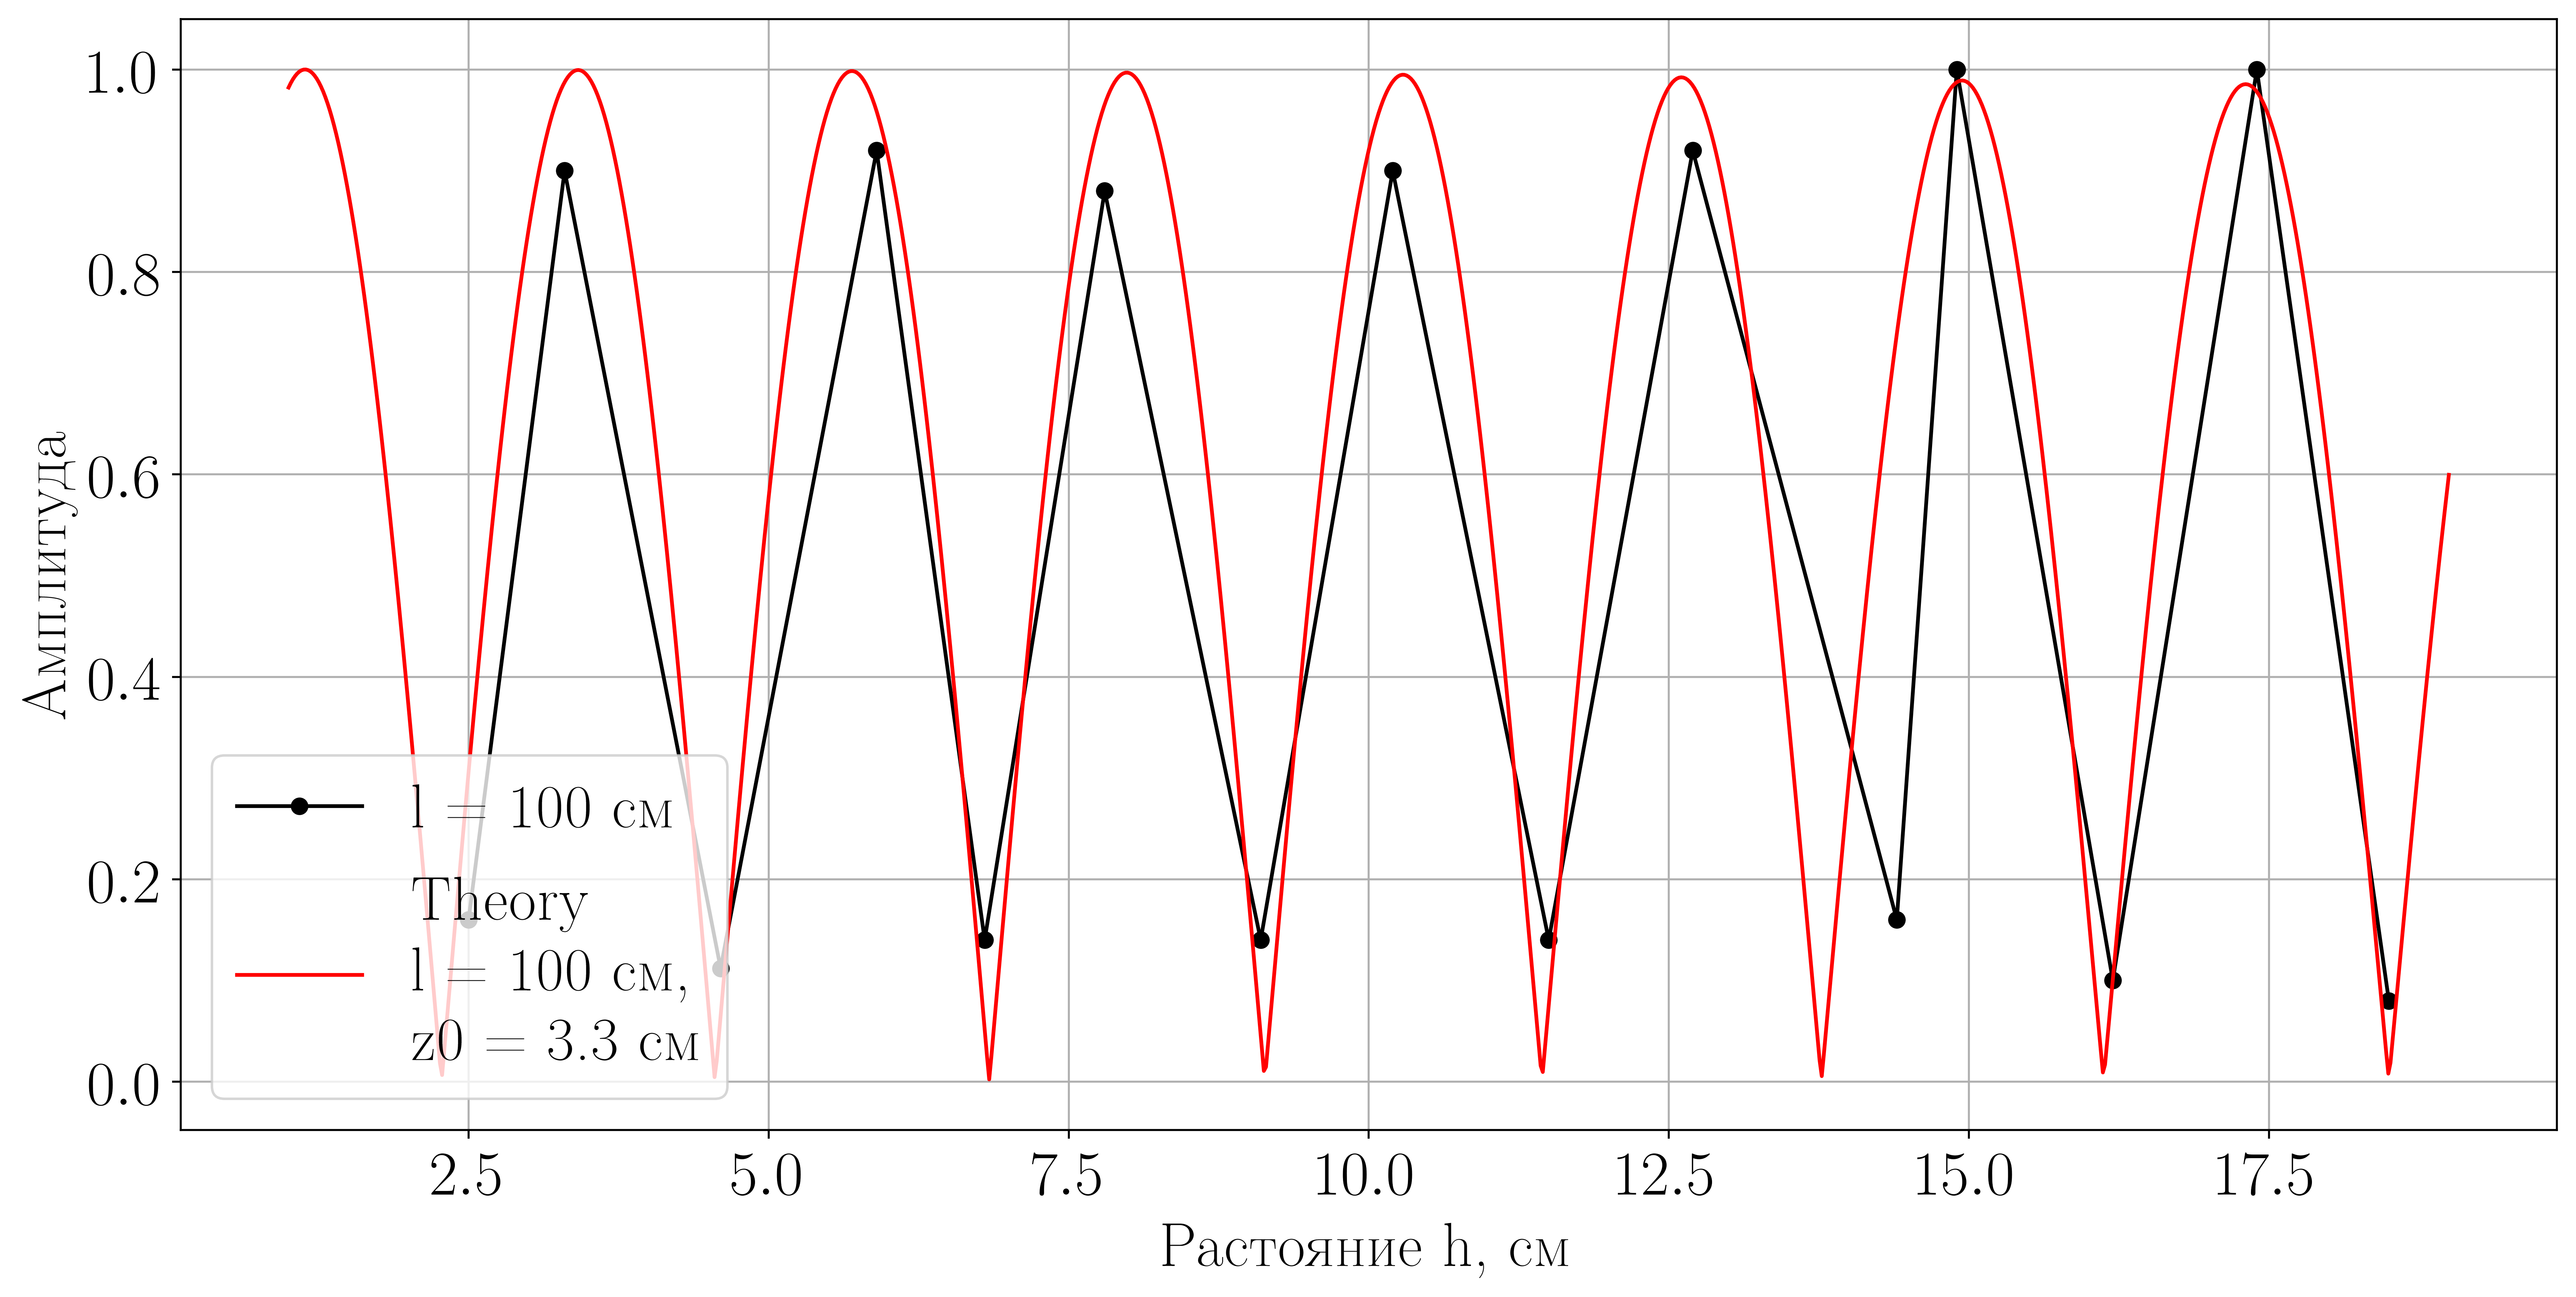
\includegraphics[width =0.79\linewidth]{fig/task32}
	\caption{Амплитуды при вертикальном срезе, на расстоянии $l=100$ см}
	\label{fig:task32}
\end{figure}

\begin{figure}[h!]
	\centering
	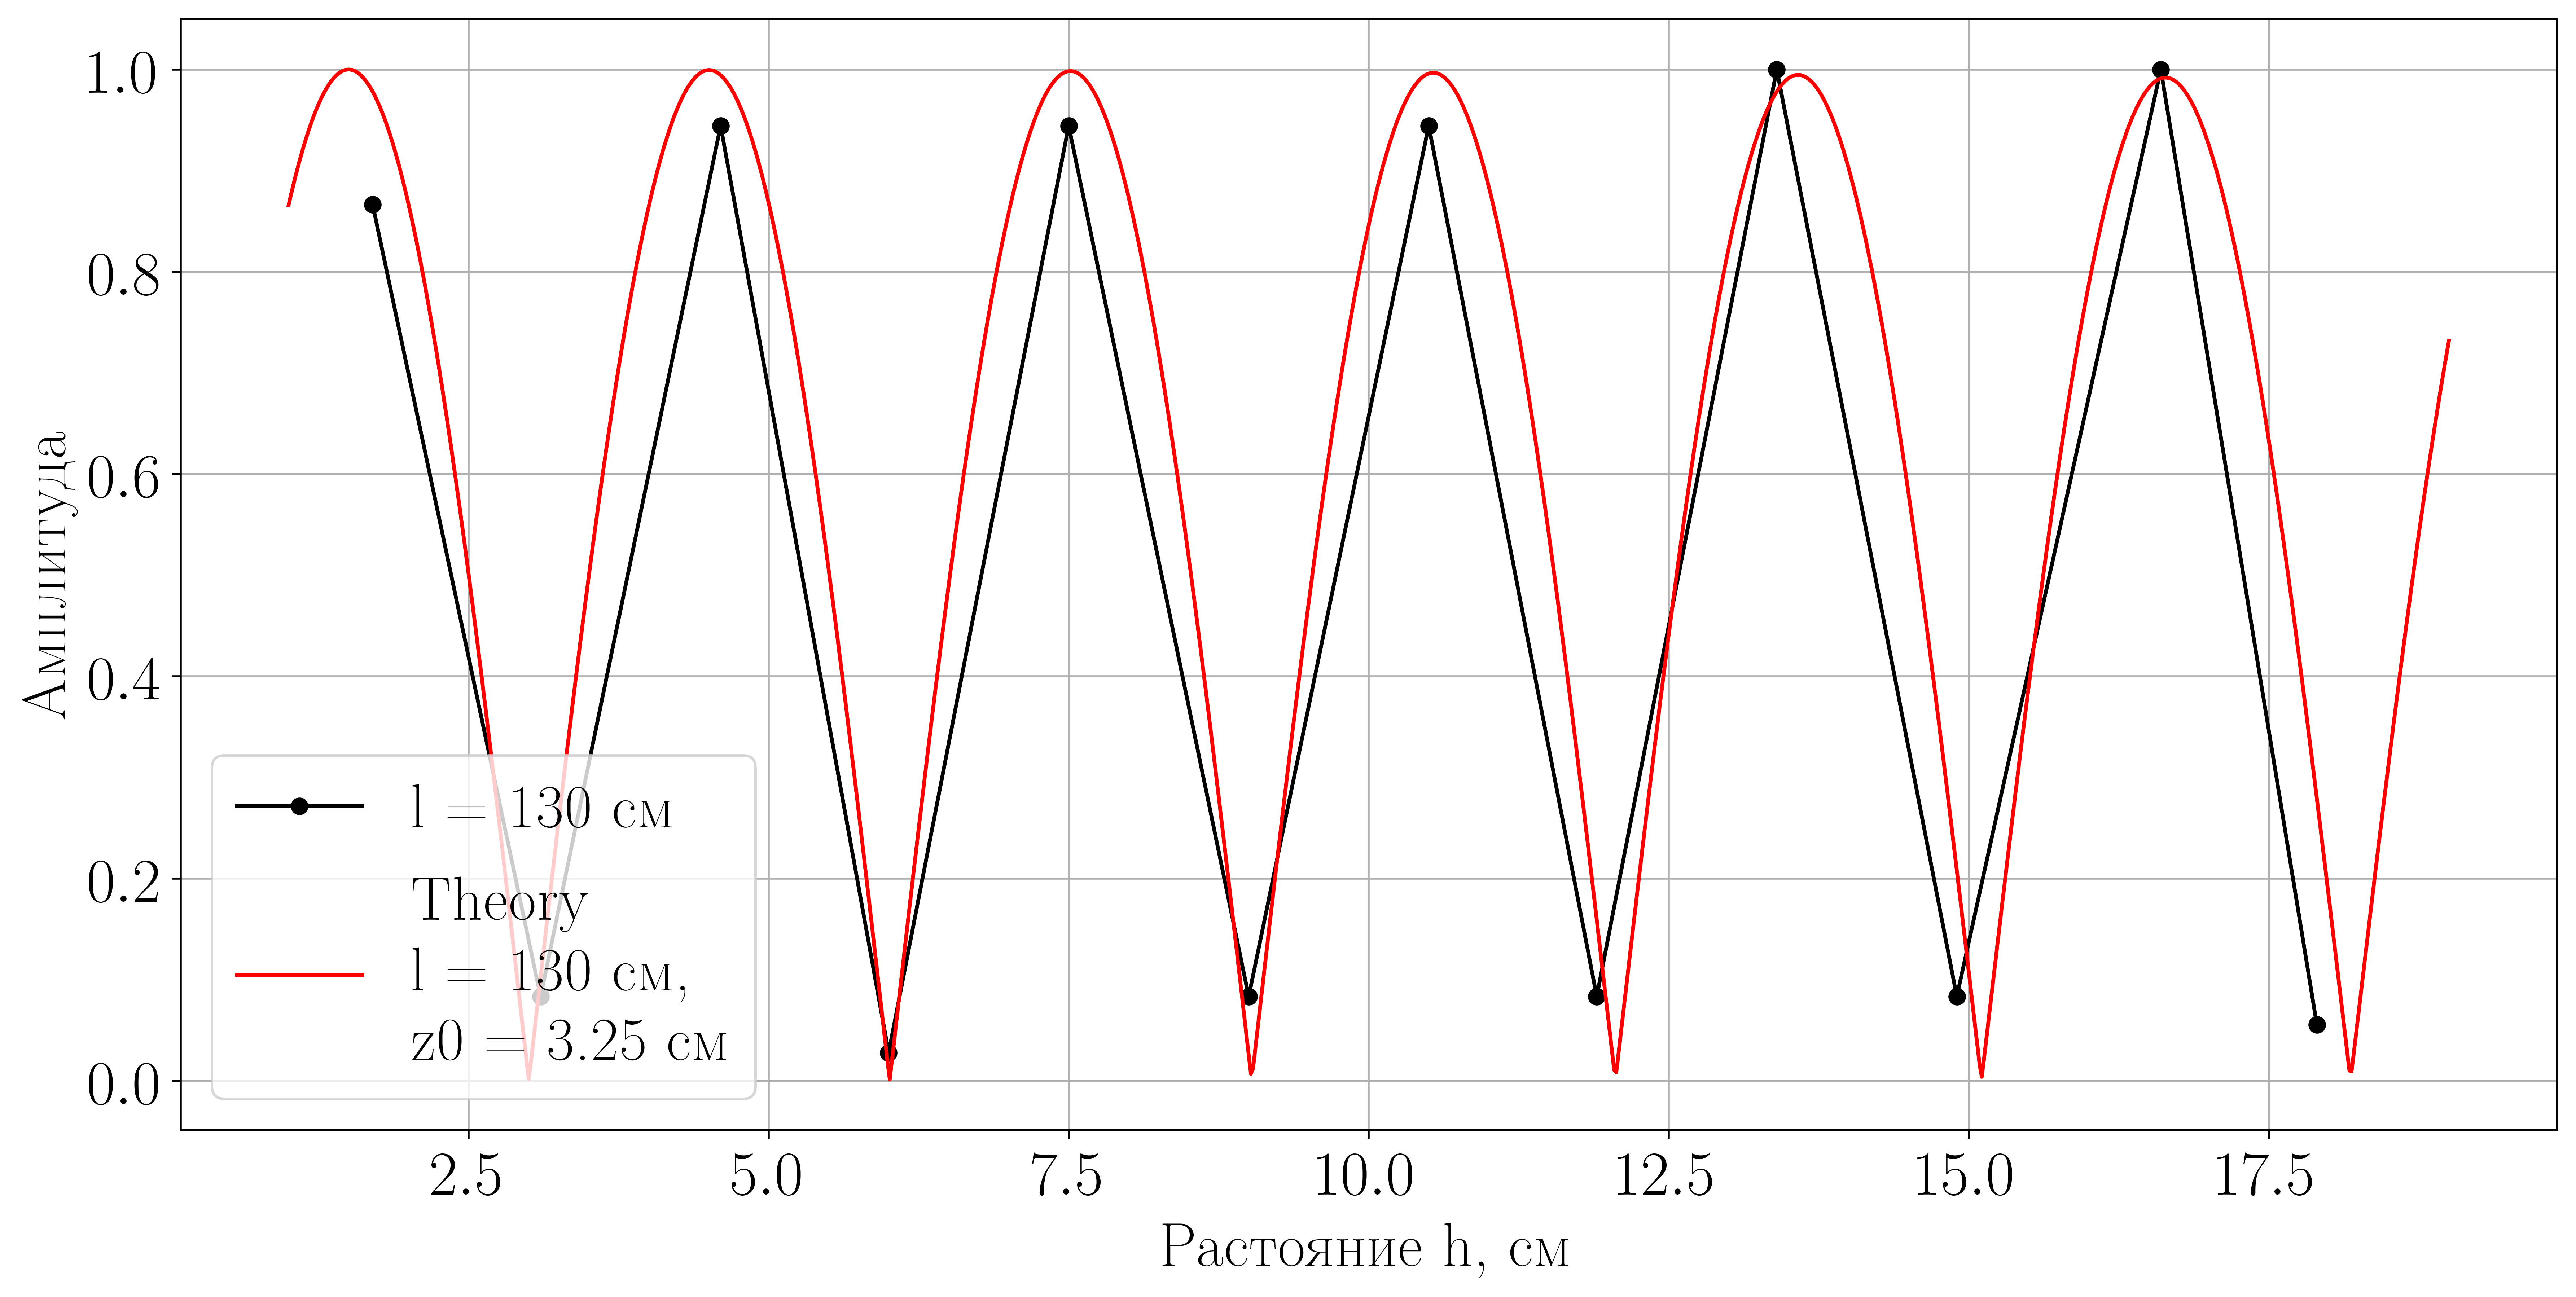
\includegraphics[width =0.79\linewidth]{fig/task33}
	\caption{Амплитуды при вертикальном срезе, на расстоянии $l=130$ см}
	\label{fig:task33}
\end{figure}

Амплитуды максимумов и минимумов для вертикальных срезов приведены на рис. \ref{fig:task31}, \ref{fig:task32},
\ref{fig:task33}.
Полученные экспериментально вертикальные срезы также достаточно хорошо совпадают с теоретическими ожаданиями. Чем дальше
от источника проводились измерения, тем реже чередовались минимумы и максимумы. При это частота чередования менялась
мало, что свидетельствует о достаточно большой плотности лепестков диаграммы направленности системы из реального и
мнимого источника.

\subsection{Определение добротности пьезо-излучателя}

Для определения добротности излучателя $Q$, была зафиксирована осциллограмма принимаемого сигнала, приведенная на рис.
\ref{fig:Q1}. Как видно в начале и в конце наблюдаются искажения формы импульса, что связано с инертностью мембраны
пьезо-излучателя. 

\begin{figure}[h!]
	\centering
	\begin{minipage}{0.49\linewidth}
		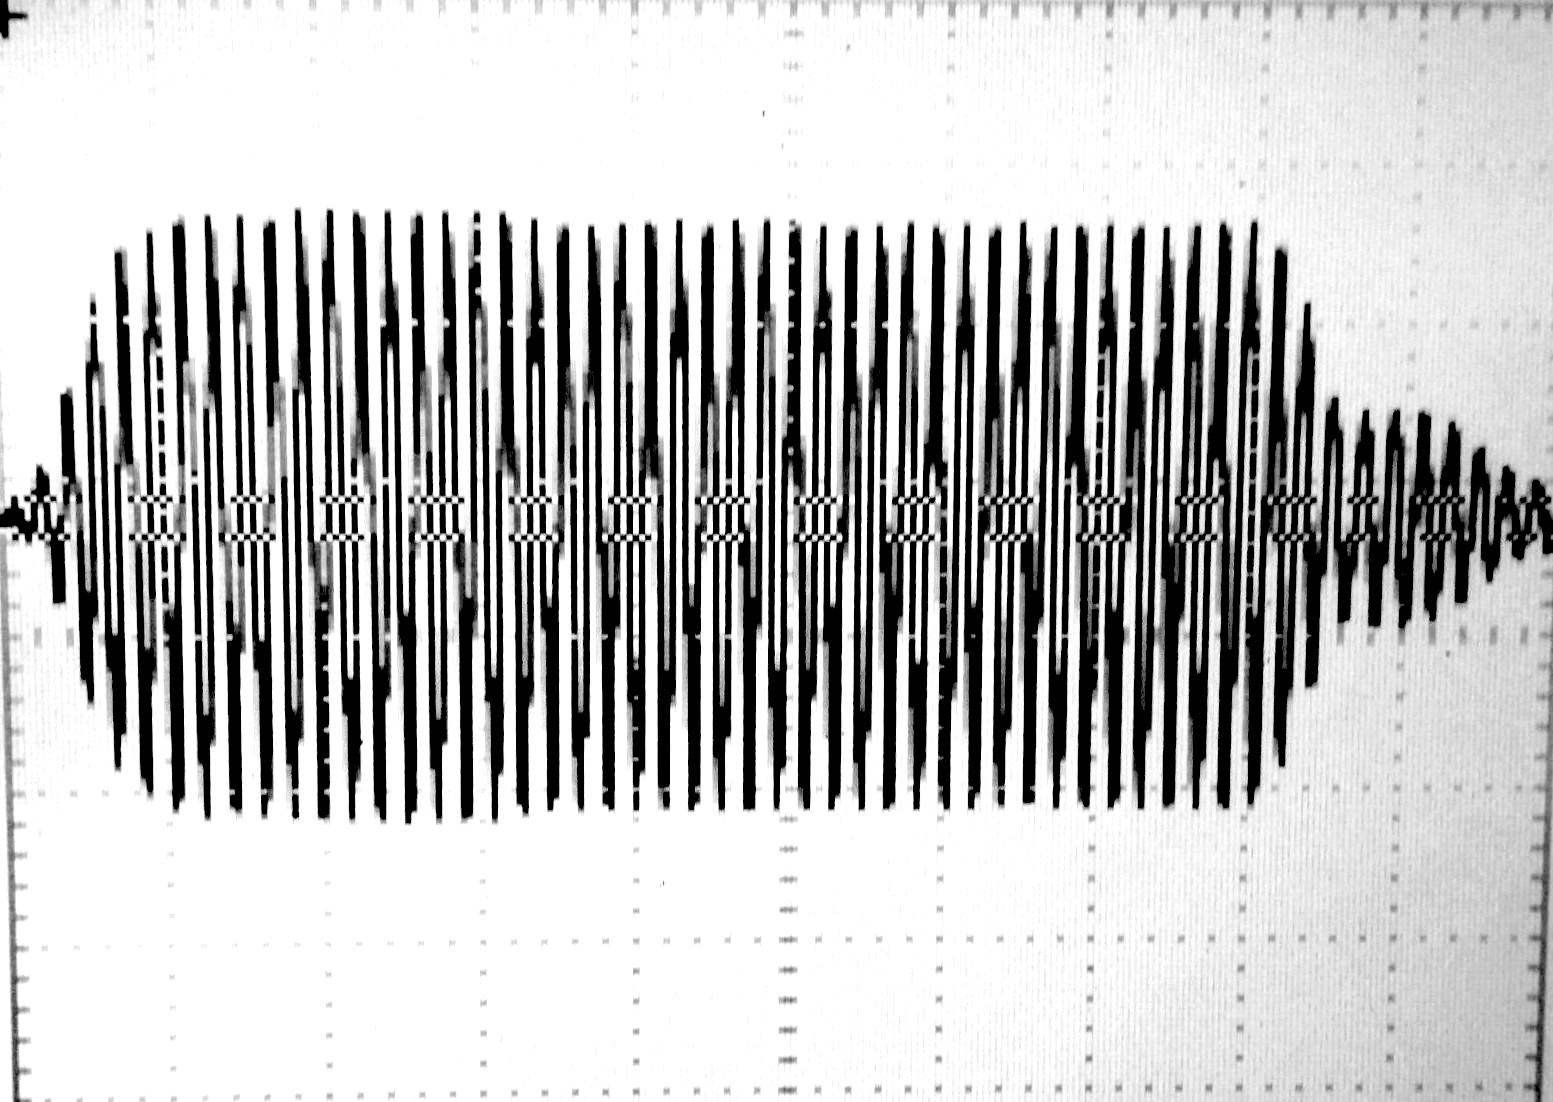
\includegraphics[width =\linewidth]{fig/Q/1.jpg}
		\caption{Осциллограмма принимаемого импульса}
		\label{fig:Q1}
	\end{minipage}
	\begin{minipage}{0.49\linewidth}
		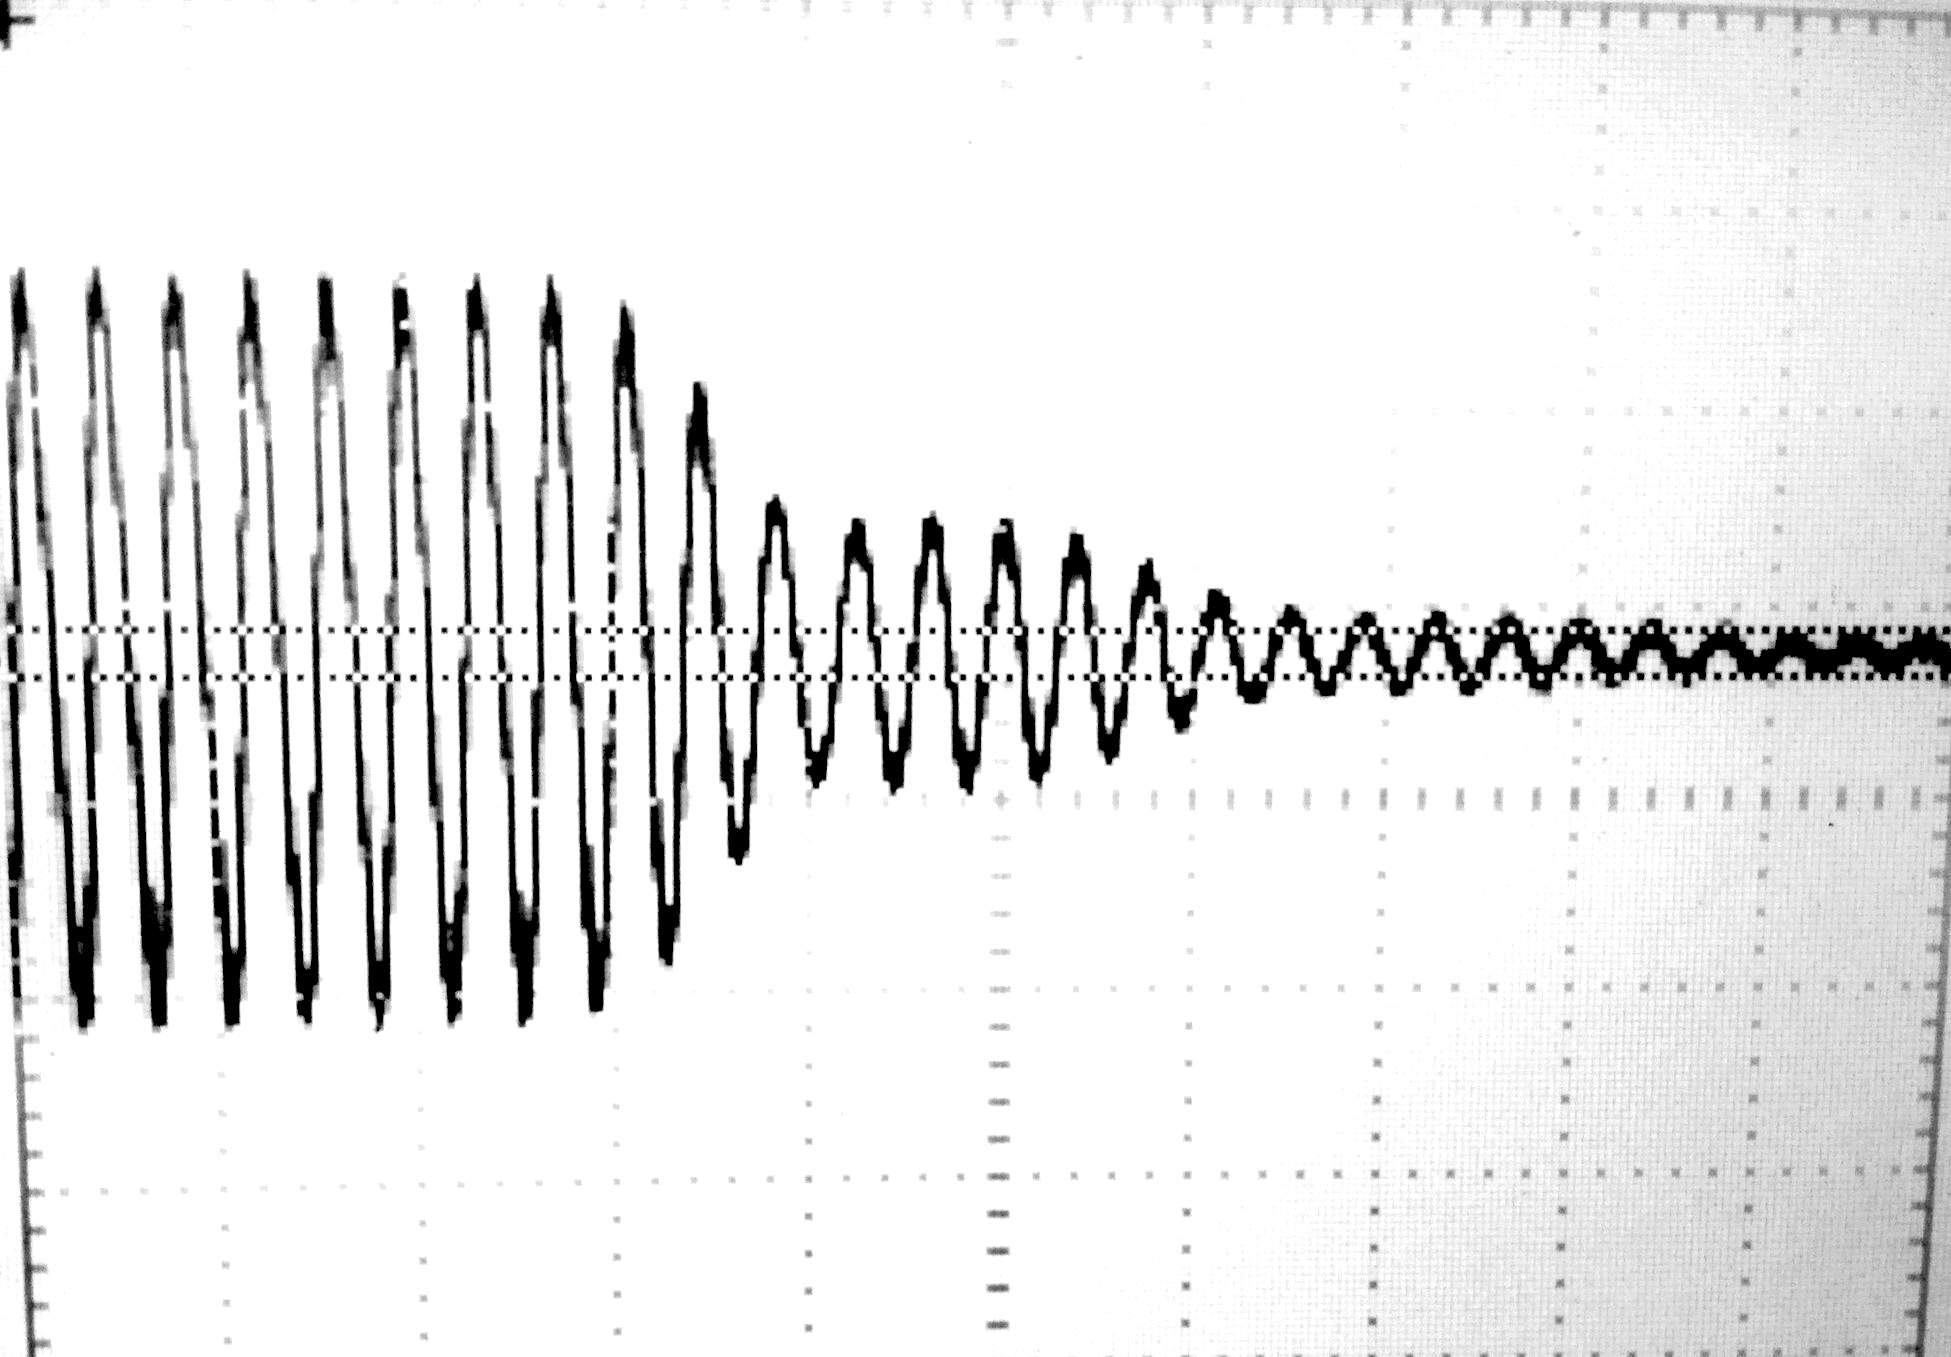
\includegraphics[width =\linewidth]{fig/Q/3.jpg}
		\caption{Осциллограмма окончания принимаемого импульса}
		\label{fig:Q2}
	\end{minipage}
\end{figure}

Для определения добротности $Q$ воспользуемся формулой 
\begin{equation}
	Q = \pi N_e,
	\label{eq:dobr}
\end{equation}
где $N_e$ - число колебаний за время релаксации. Подробнее рассмотрим принимаемый импульс, а именно количество затухающих
колебаний за время релаксации (см. рис. \ref{fig:Q2}). В конце импульса количество колебаний $N_e = 8$, добротность
в таком случае $Q \simeq 25.2$


\end{document}
